\documentclass[11pt,xcolor=dvipsnames,aspectratio=169]{beamer}

\mode<presentation>
{
  \useinnertheme{circles} 
  \usecolortheme[named=Black]{structure} 
  \setbeamertemplate{navigation symbols}{}
  \setbeamertemplate{footline}[page number]
  \setbeamercovered{transparent}
}

\usepackage{physcomm}

%\usepackage{adjustbox}
\usepackage[export]{adjustbox}
\usepackage{graphicx}
\usepackage{colortbl}
\usepackage{pifont}
\usepackage{amsmath}
\usepackage{scrdate,scrtime}
\usepackage{subfig}
\usepackage{verbatim}
\usepackage{booktabs}
\usepackage{rotating}
\usepackage{xspace}
\usepackage{xcolor}
\usepackage{bm}
\usepackage{pdfpages}
\usepackage{enumerate}
\usepackage{amsmath}
\usepackage{xspace}
\usepackage{ifthen}
 
%-----------------------------------------------------------------------
% custom colors 
\definecolor{EDBRed}{RGB}{220,20,60} 
\definecolor{EDBDarkBlue}{RGB}{0,0,160}
\definecolor{EDBBlue}{RGB}{0,135,189}
\definecolor{EDBGray}{RGB}{211,211,211}

%-----------------------------------------------------------------------
% text boxes 
\usepackage{tcolorbox}
%\usepackage{mdframed}

% 1- Block title (background and text)
\setbeamercolor{block title}{bg=EDBBlue!60, fg=black}
% 2- Block body (background)
\setbeamercolor{block body}{bg=EDBBlue!60}

\setbeamercolor{block title alerted}{fg=white, bg=orange}
% 2- Block body (background)
\setbeamercolor{block body alerted}{bg=orange!25}

% 1- Block title (background and text)
\setbeamercolor{block title example}{fg=white, bg=teal}
% 2- Block body (background and text)
\setbeamercolor{block body example}{bg=EDBBlue!60}

% arrows between color boxes
\usepackage{tikz}
\usetikzlibrary{arrows.meta, % for arrows style
                positioning  % for positioning of boxes
               }

%-----------------------------------------------------------------------
% backup 
\newcommand{\backupbegin}{
   \newcounter{framenumberappendix}
   \setcounter{framenumberappendix}{\value{framenumber}}
    \setbeamertemplate{footline}{
   \leavevmode%
   \hbox{%
   \begin{beamercolorbox}[wd=1.00\paperwidth,ht=0.01ex,dp=1ex,right]{} 
     {\normalsize \insertframenumber{}} \hspace{0.065\textwidth}
   \end{beamercolorbox}
   }%
   \vskip0pt%
 }
}

\newcommand{\backupend}{
   \addtocounter{framenumberappendix}{-\value{framenumber}}
   \addtocounter{framenumber}{\value{framenumberappendix}} 
}

% -----------------------------------------------------------------------
% slide layout & footnotes
\setbeamertemplate{frametitle}{ 
%\begin{centering} 
\vspace{0.03\paperheight}
{\huge \insertframetitle }
\vspace{0.01\paperheight}
\par 
%\end{centering} 
}


%\setbeamertemplate{footline}[text line]{%
%\parbox{\linewidth}{\small \vspace*{-10pt} \ \hfill \ \insertpagenumber / \inserttotalframenumber}}

\setbeamertemplate{footline}[text line]{%
\parbox{\linewidth}{\small \vspace*{-10pt} \ \hfill \ \insertframenumber / \inserttotalframenumber}}

\let\footnoterule\relax

\newcommand\blfootnote[1]{%
  \begingroup
  \renewcommand\thefootnote{}\footnote{\hspace{-30pt}\textcolor{Gray}{\tiny #1}}%
  \addtocounter{footnote}{-1}%
  \endgroup
}

% -----------------------------------------------------------------------
% itemize margins
\setlength{\leftmargini}{0.025\linewidth}
\setlength{\leftmarginii}{0.021\linewidth}

% sub-item size:
\setbeamerfont{itemize/enumerate subbody}{size=\normalsize} %to set the body size
%\setbeamertemplate{itemize subitem}{\normalsize\raise1.25pt\hbox{\donotcoloroutermaths$\blacktriangleright$}}  %to set the symbol size 
% -----------------------------------------------------------------------
\begin{document}

{
\usebackgroundtemplate{
\includegraphics[width=\paperwidth]{background/template_169_logos.pdf}}%
\begin{frame}[noframenumbering,plain]
  \begin{center}
    \setlength{\parskip}{0pt}
    \vspace{10pt}
    {\Huge\bf Deep Learning \& the Higgs Boson}\\[0.1\textheight]
    {\huge \bf Dr. Liza Mijovi\'c}
  \end{center}
\end{frame}
}

{
\usebackgroundtemplate{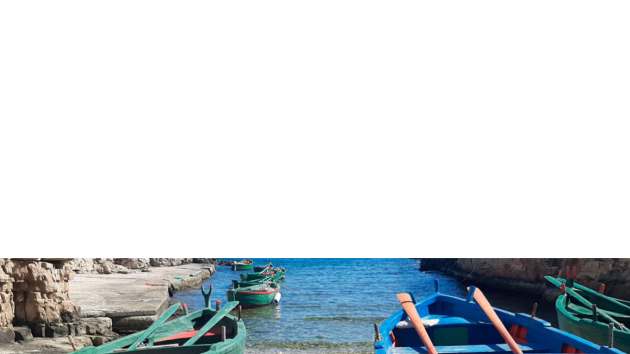
\includegraphics[width=\paperwidth]{background/template_169.pdf}}%
\begin{frame}[plain]
  \frametitle{\bf Deep Learning \& the Higgs Boson}
  \adjustbox{valign=t}{\begin{minipage}[t][0.55\textheight]{\linewidth}
      Classification with Fully Connected and Adversarial Networks.
      \vfill
      \begin{itemize}
      \item {\bf Lecture1: The Higgs boson and event classification:}\\
        - Event classification with a fully connected neural network (NN) with Keras API.\\
      \end{itemize}
      \vfill
      \begin{itemize}      
      \item {\bf Lecture2: Solving the background sculpting challenge:}\\
        - Event classification with adversarial neural network (ANN).\\
        - Hands-on knowledge of manipulating neural networks in Tensorflow.
      \end{itemize}
      \vfill
      \begin{itemize}          
      \item {\bf Lecture3: Putting it all together:}\\
        - Compare ANN classification performance to the fully connected network.
      \end{itemize}
      \vfill
\end{minipage}}
% vertical place-holder
\adjustbox{valign=t}{\begin{minipage}[t][0.35\textheight]{\linewidth} 
  \end{minipage}}
\end{frame}
}


\begin{frame}[plain]
  \frametitle{\bf Lecture Schedule}
     \adjustbox{valign=c}{\begin{minipage}[c]{0.6\linewidth}   
         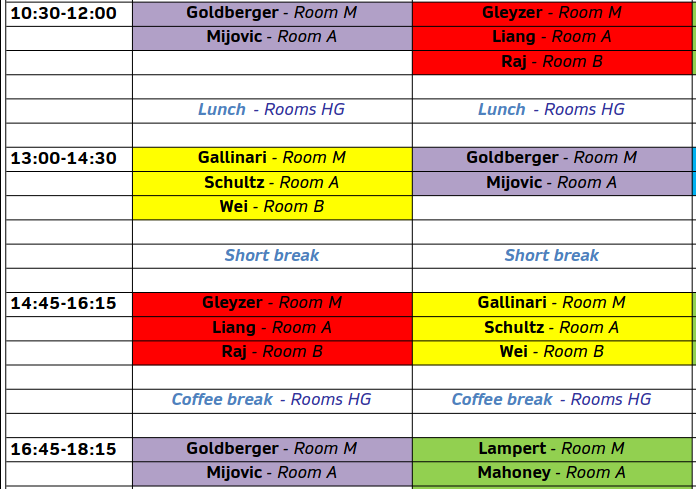
\includegraphics[width=1.00\textwidth]{figures/l1/schedule.png}
     \end{minipage}}
     \hfill
     \adjustbox{valign=c}{\begin{minipage}[c]{0.34\linewidth}
         {\bf Room A:}
         \vfill
          \begin{itemize}
            \item {\bf Lecture1: Mon Morning}
          \end{itemize}
          \begin{itemize}
            \item {\bf Lecture2: Mon Evening}
          \end{itemize}
          \begin{itemize}
            \item {\bf Lecture3: Tue Afternoon}
          \end{itemize}
          \vfill
          {\bf Please bring your laptop.}
     \end{minipage}}
\end{frame}


{
\usebackgroundtemplate{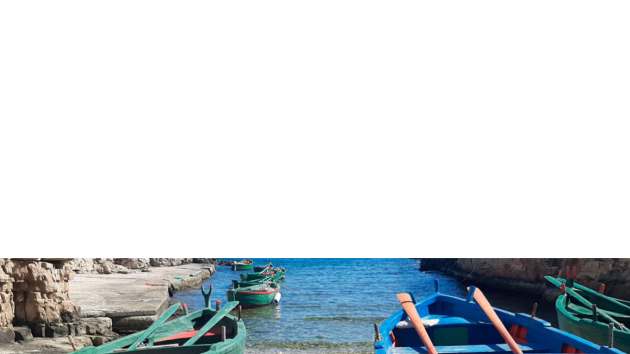
\includegraphics[width=\paperwidth]{background/template_169.pdf}}%
\begin{frame}[plain]
  \frametitle{}
  \adjustbox{valign=t}{\begin{minipage}[t][0.55\textheight]{\linewidth}
      \vfill
      \begin{center}
      {\bf \Huge Lecture1:\\[2ex] Higgs boson \& event classification:}\\[2ex]
        {\Large event classification with a fully connected neural network (NN) with Keras API.}\\
      \end{center}
      \vfill
\end{minipage}}
% vertical place-holder
\adjustbox{valign=t}{\begin{minipage}[t][0.35\textheight]{\linewidth} 
  \end{minipage}}
\end{frame}
}

\begin{frame}[fragile]
  \frametitle{\bf Fundamental Particles and Collisions}
  \begin{figure}
    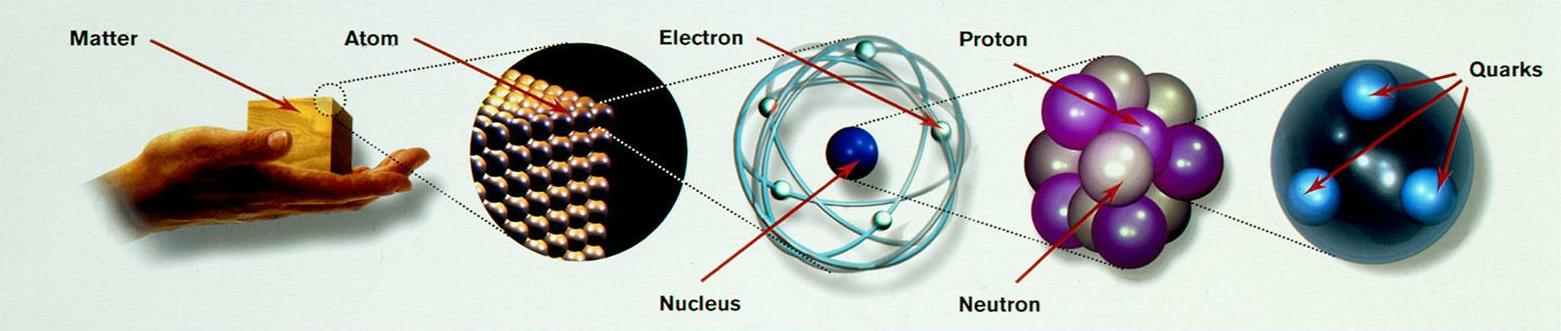
\includegraphics[width=1.0\textwidth]{figures/l1/intro/atom_to_quark.png}
  \end{figure}
  
  \adjustbox{valign=t}{\begin{minipage}[c]{0.5\linewidth} 
      \begin{figure}
        \includegraphics[width=1.00\textwidth]{figures/l1/intro/lhc_coll.png}
      \end{figure}
    \end{minipage}}
  \hfill
  \adjustbox{valign=t}{\begin{minipage}[c]{0.44\linewidth}
      \vspace{10pt}
      {\bf Large Hadron Collider (LHC):}
      \begin{itemize}
      \item {\bf Collide protons.}
      \end{itemize}
      \begin{itemize}
      \item {\bf New particles:} $\bm{\mathrm{E}} \bm{\sim} \bm{\mathrm{mc}}^{\bm 2}${\bf .}
      \end{itemize}
      \begin{itemize}
      \item {\bf Detector: snap-shot of collision.}
      \end{itemize}
    \end{minipage}} 
\end{frame}


\begin{frame}[fragile]
  \frametitle{\bf  Why study particle collisions?}
  % . Yet we know that the SM is not the ultimate theory. It
  \vspace{-5pt}
      \begin{figure}
        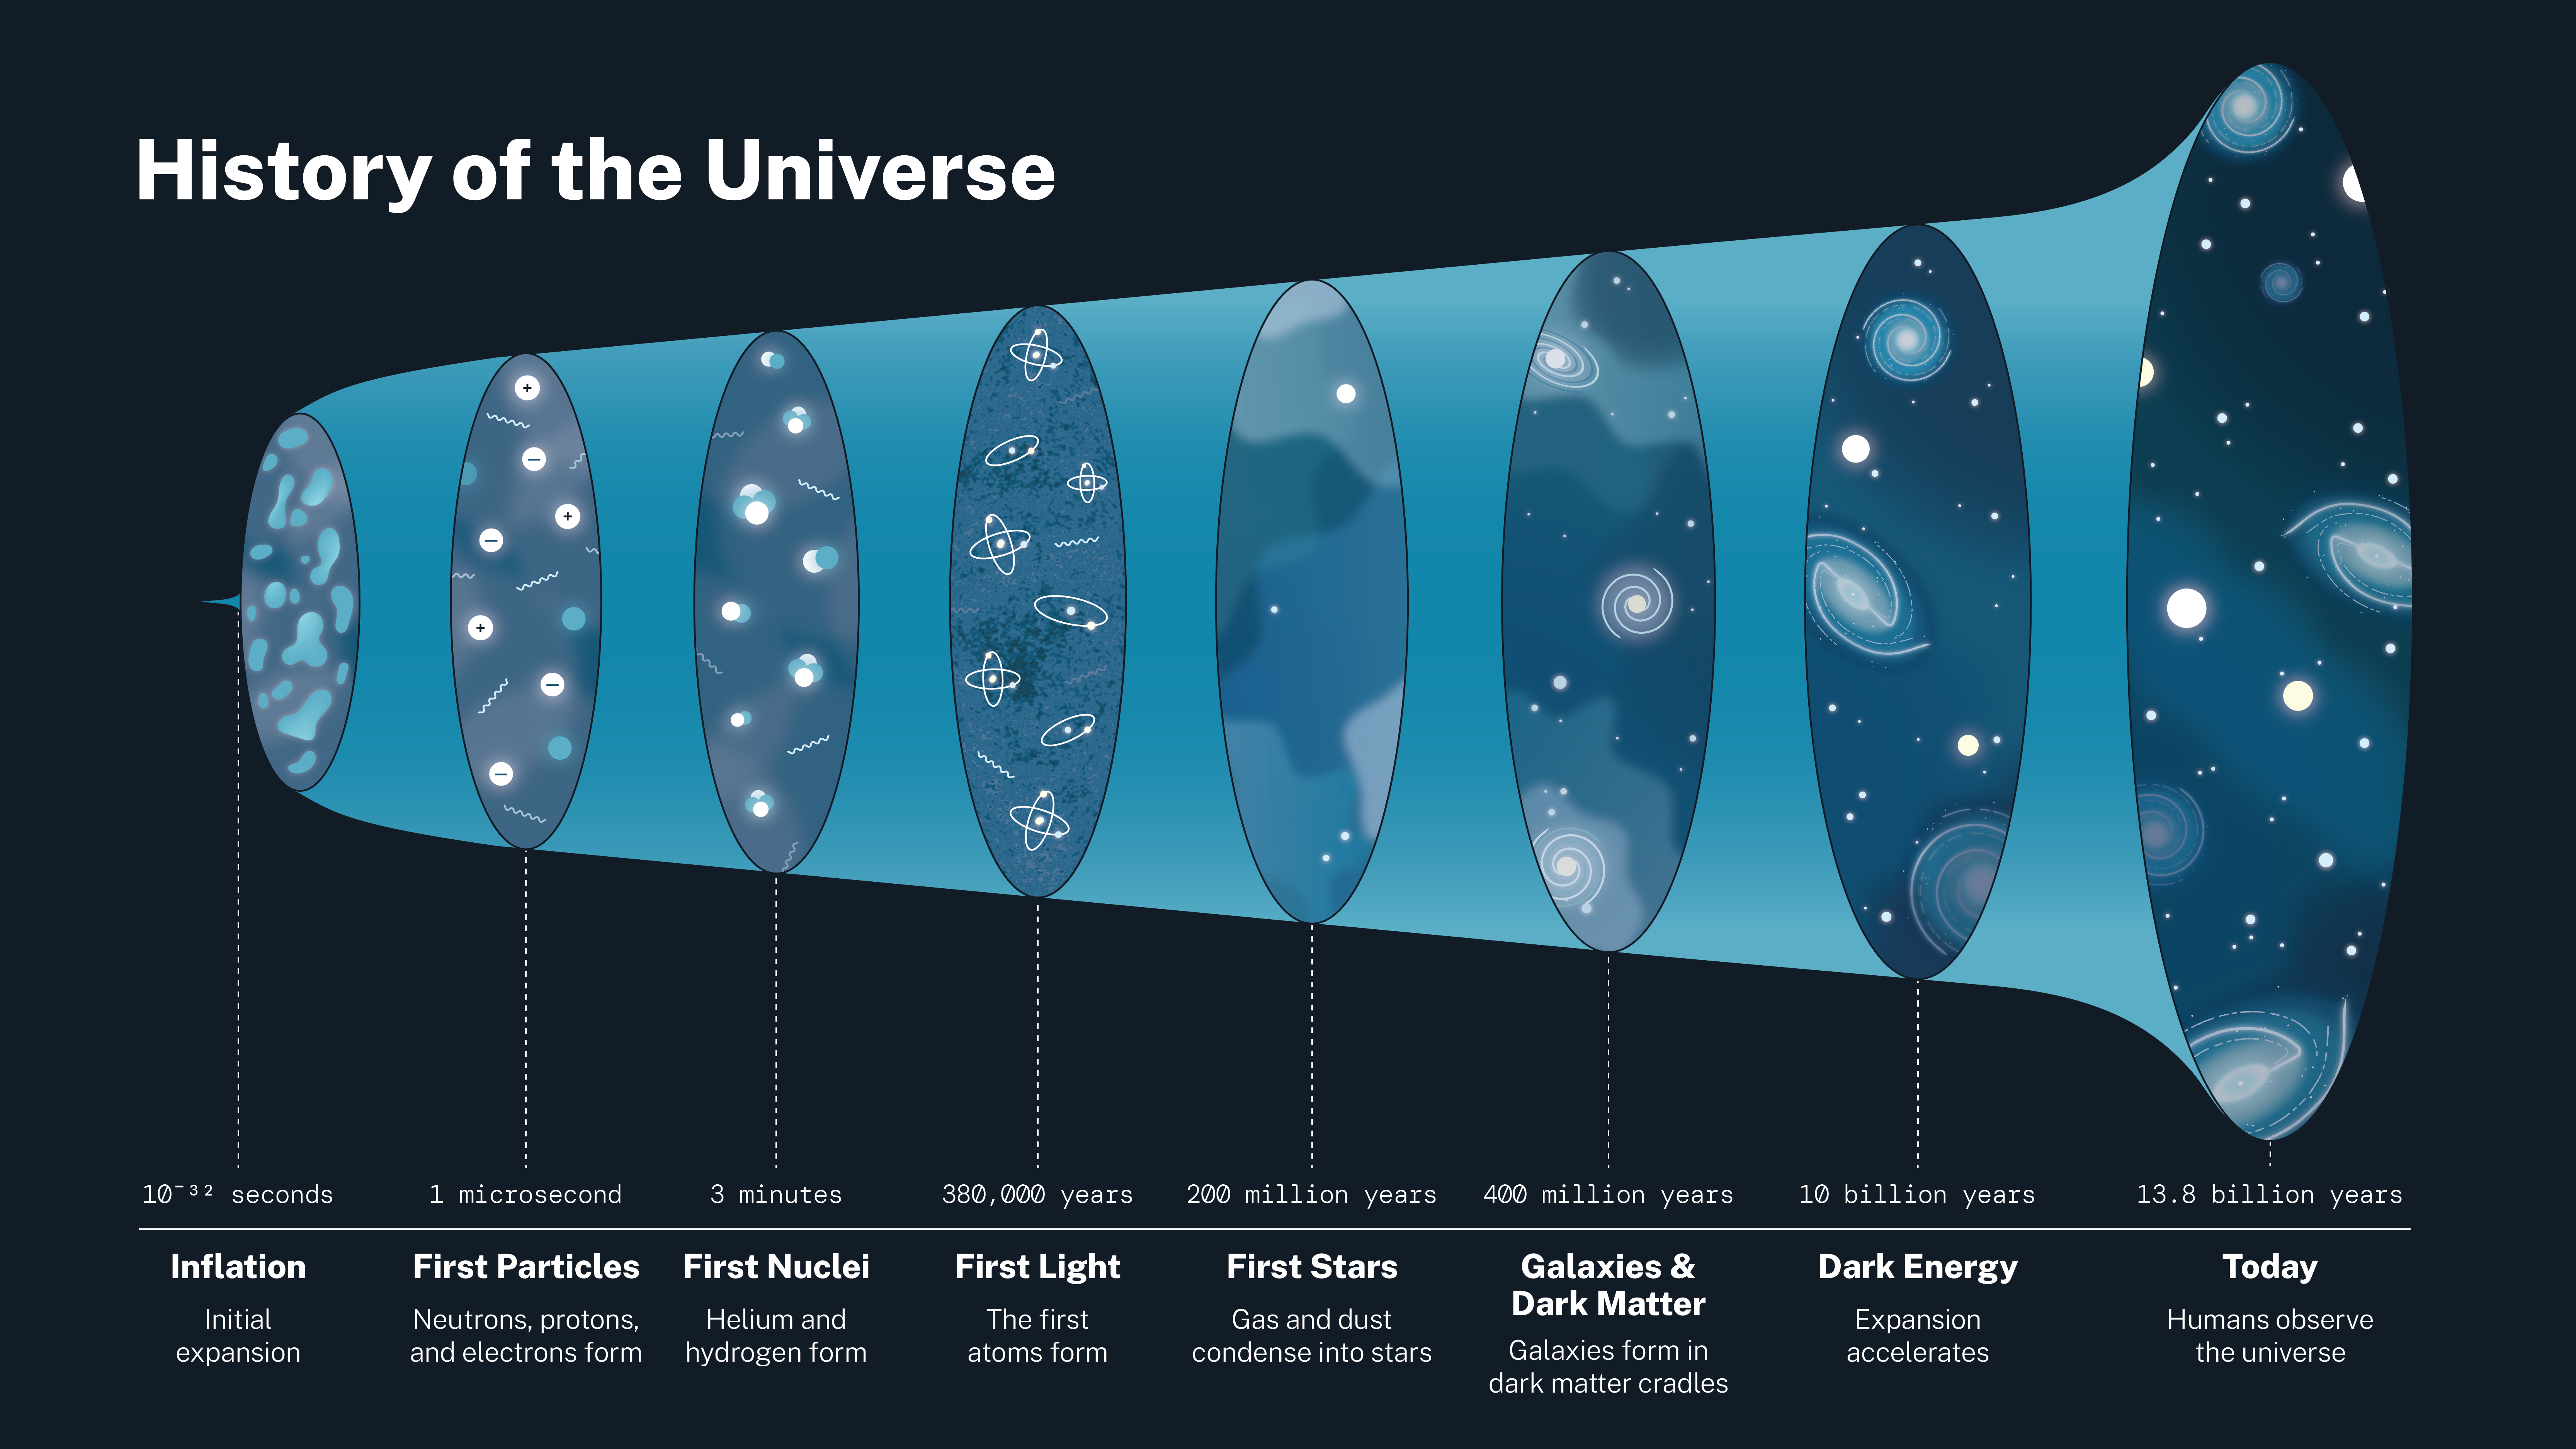
\includegraphics[width=0.85\textwidth]{figures/l1/intro/universe_nasa.png}
      \end{figure}
   \vspace{-5pt}   
      Cannot account for{$^*$}: dark matter, cosmic inflation, matter/anti-matter asymmetry. 
%      dark matter, cosmic inflation, matter/anti-matter asymmetry.
% neutrino masses,
%
%matter/anti-matter asymmetry, and , which are all experimental facts.
\blfootnote{Image
  credit: \href{https://universe.nasa.gov/universe/basics/}{NASA}.
  $^*$Additional observation we cannot account for are neutrino masses.}
    \end{frame}




\begin{frame}[fragile]
  \frametitle{\bf Challenge: Collisions are Complex}
    \adjustbox{valign=t}{\begin{minipage}[c]{0.5\linewidth} 
        \begin{figure}
          \centering
        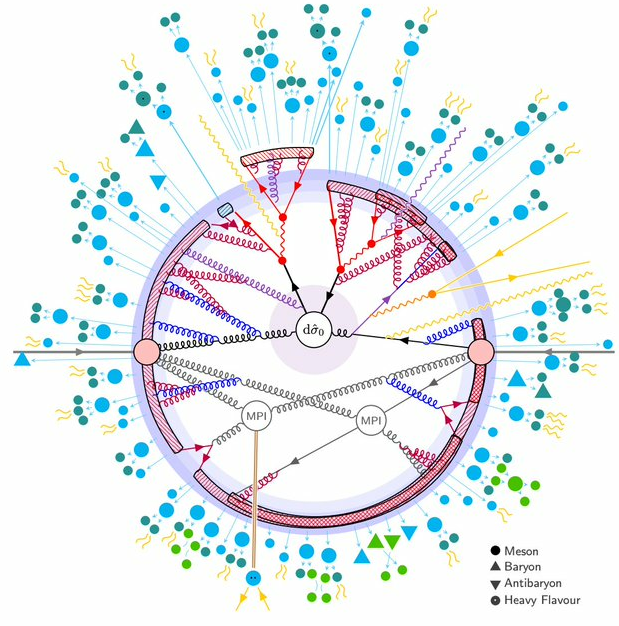
\includegraphics[width=1.00\textwidth]{figures/l1/intro/pp_nice.png}
      \end{figure}
      \end{minipage}}
    \adjustbox{valign=t}{\begin{minipage}[c]{0.49\linewidth}
      \begin{itemize}
      \item {\bf $\sim$ 1000 particles / collision.}
      \item {\bf Figure: inner-tracker.}
      \item {\bf 5B channels.}
      \end{itemize}
        
      \begin{figure}
        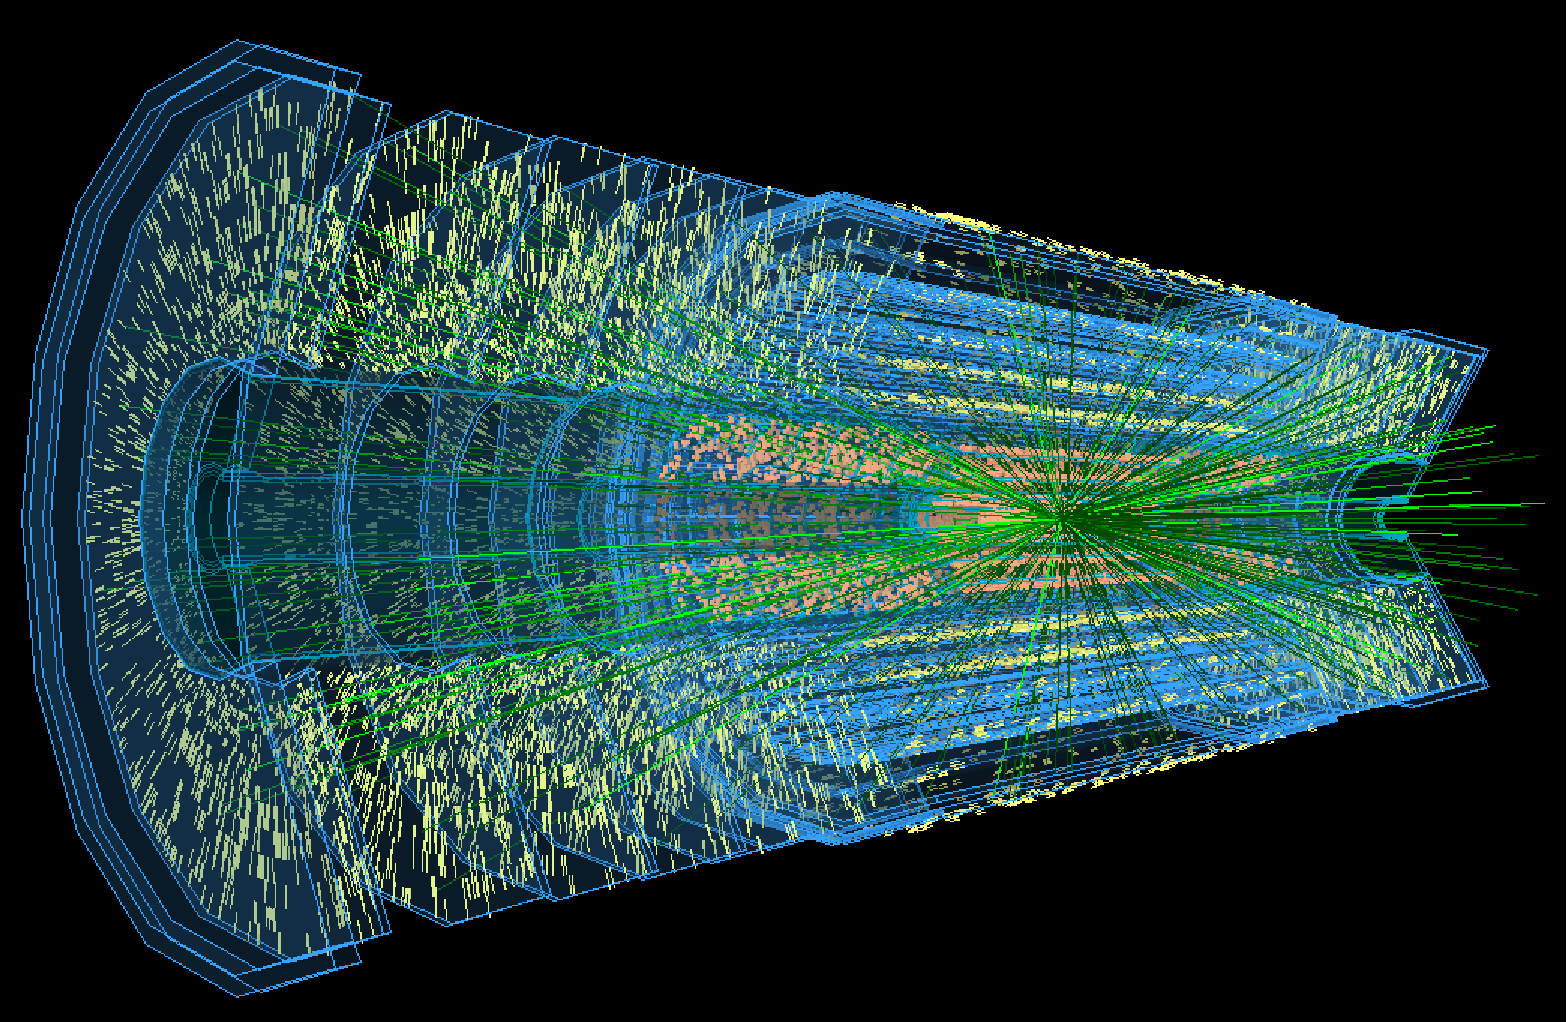
\includegraphics[width=1.00\textwidth]{figures/l1/intro/atlas-hl-lhc.png}
      \end{figure}

    \end{minipage}} 
\end{frame}

\begin{frame}[fragile]
  \frametitle{\bf LHC Detectors}
  \vspace{-5pt}
      \begin{figure}
        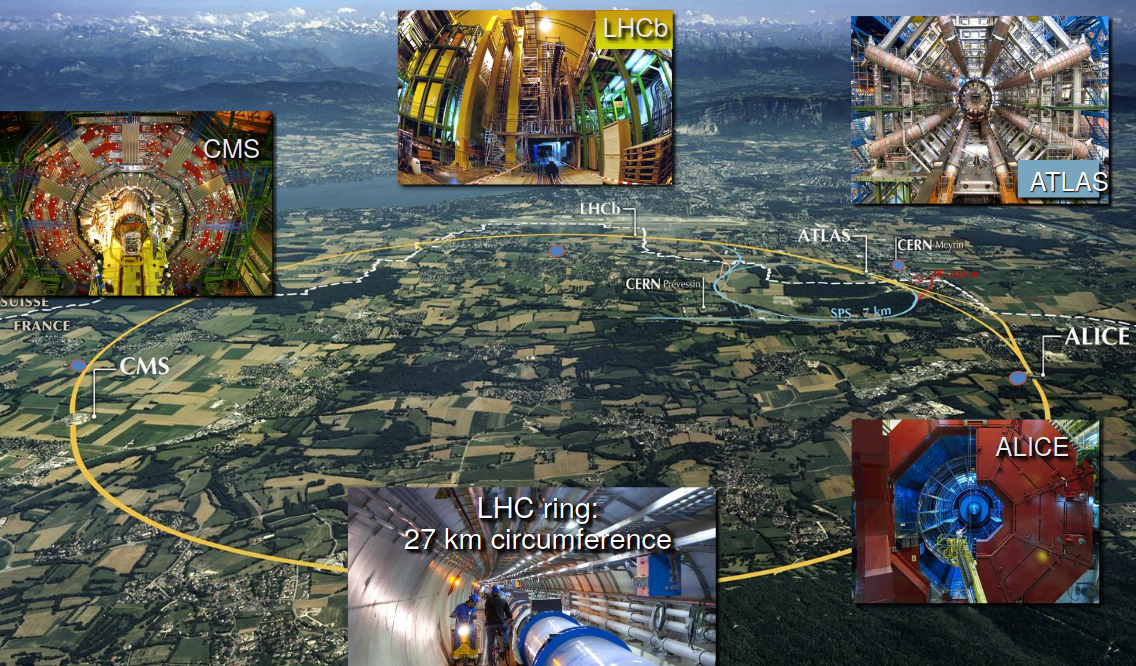
\includegraphics[width=0.90\textwidth]{figures/l1/intro/lhc_snip.png}
      \end{figure}
\end{frame}

\begin{frame}[fragile]
  \frametitle{\bf The Standard Model}
  \vspace{-5pt}
      \begin{figure}
        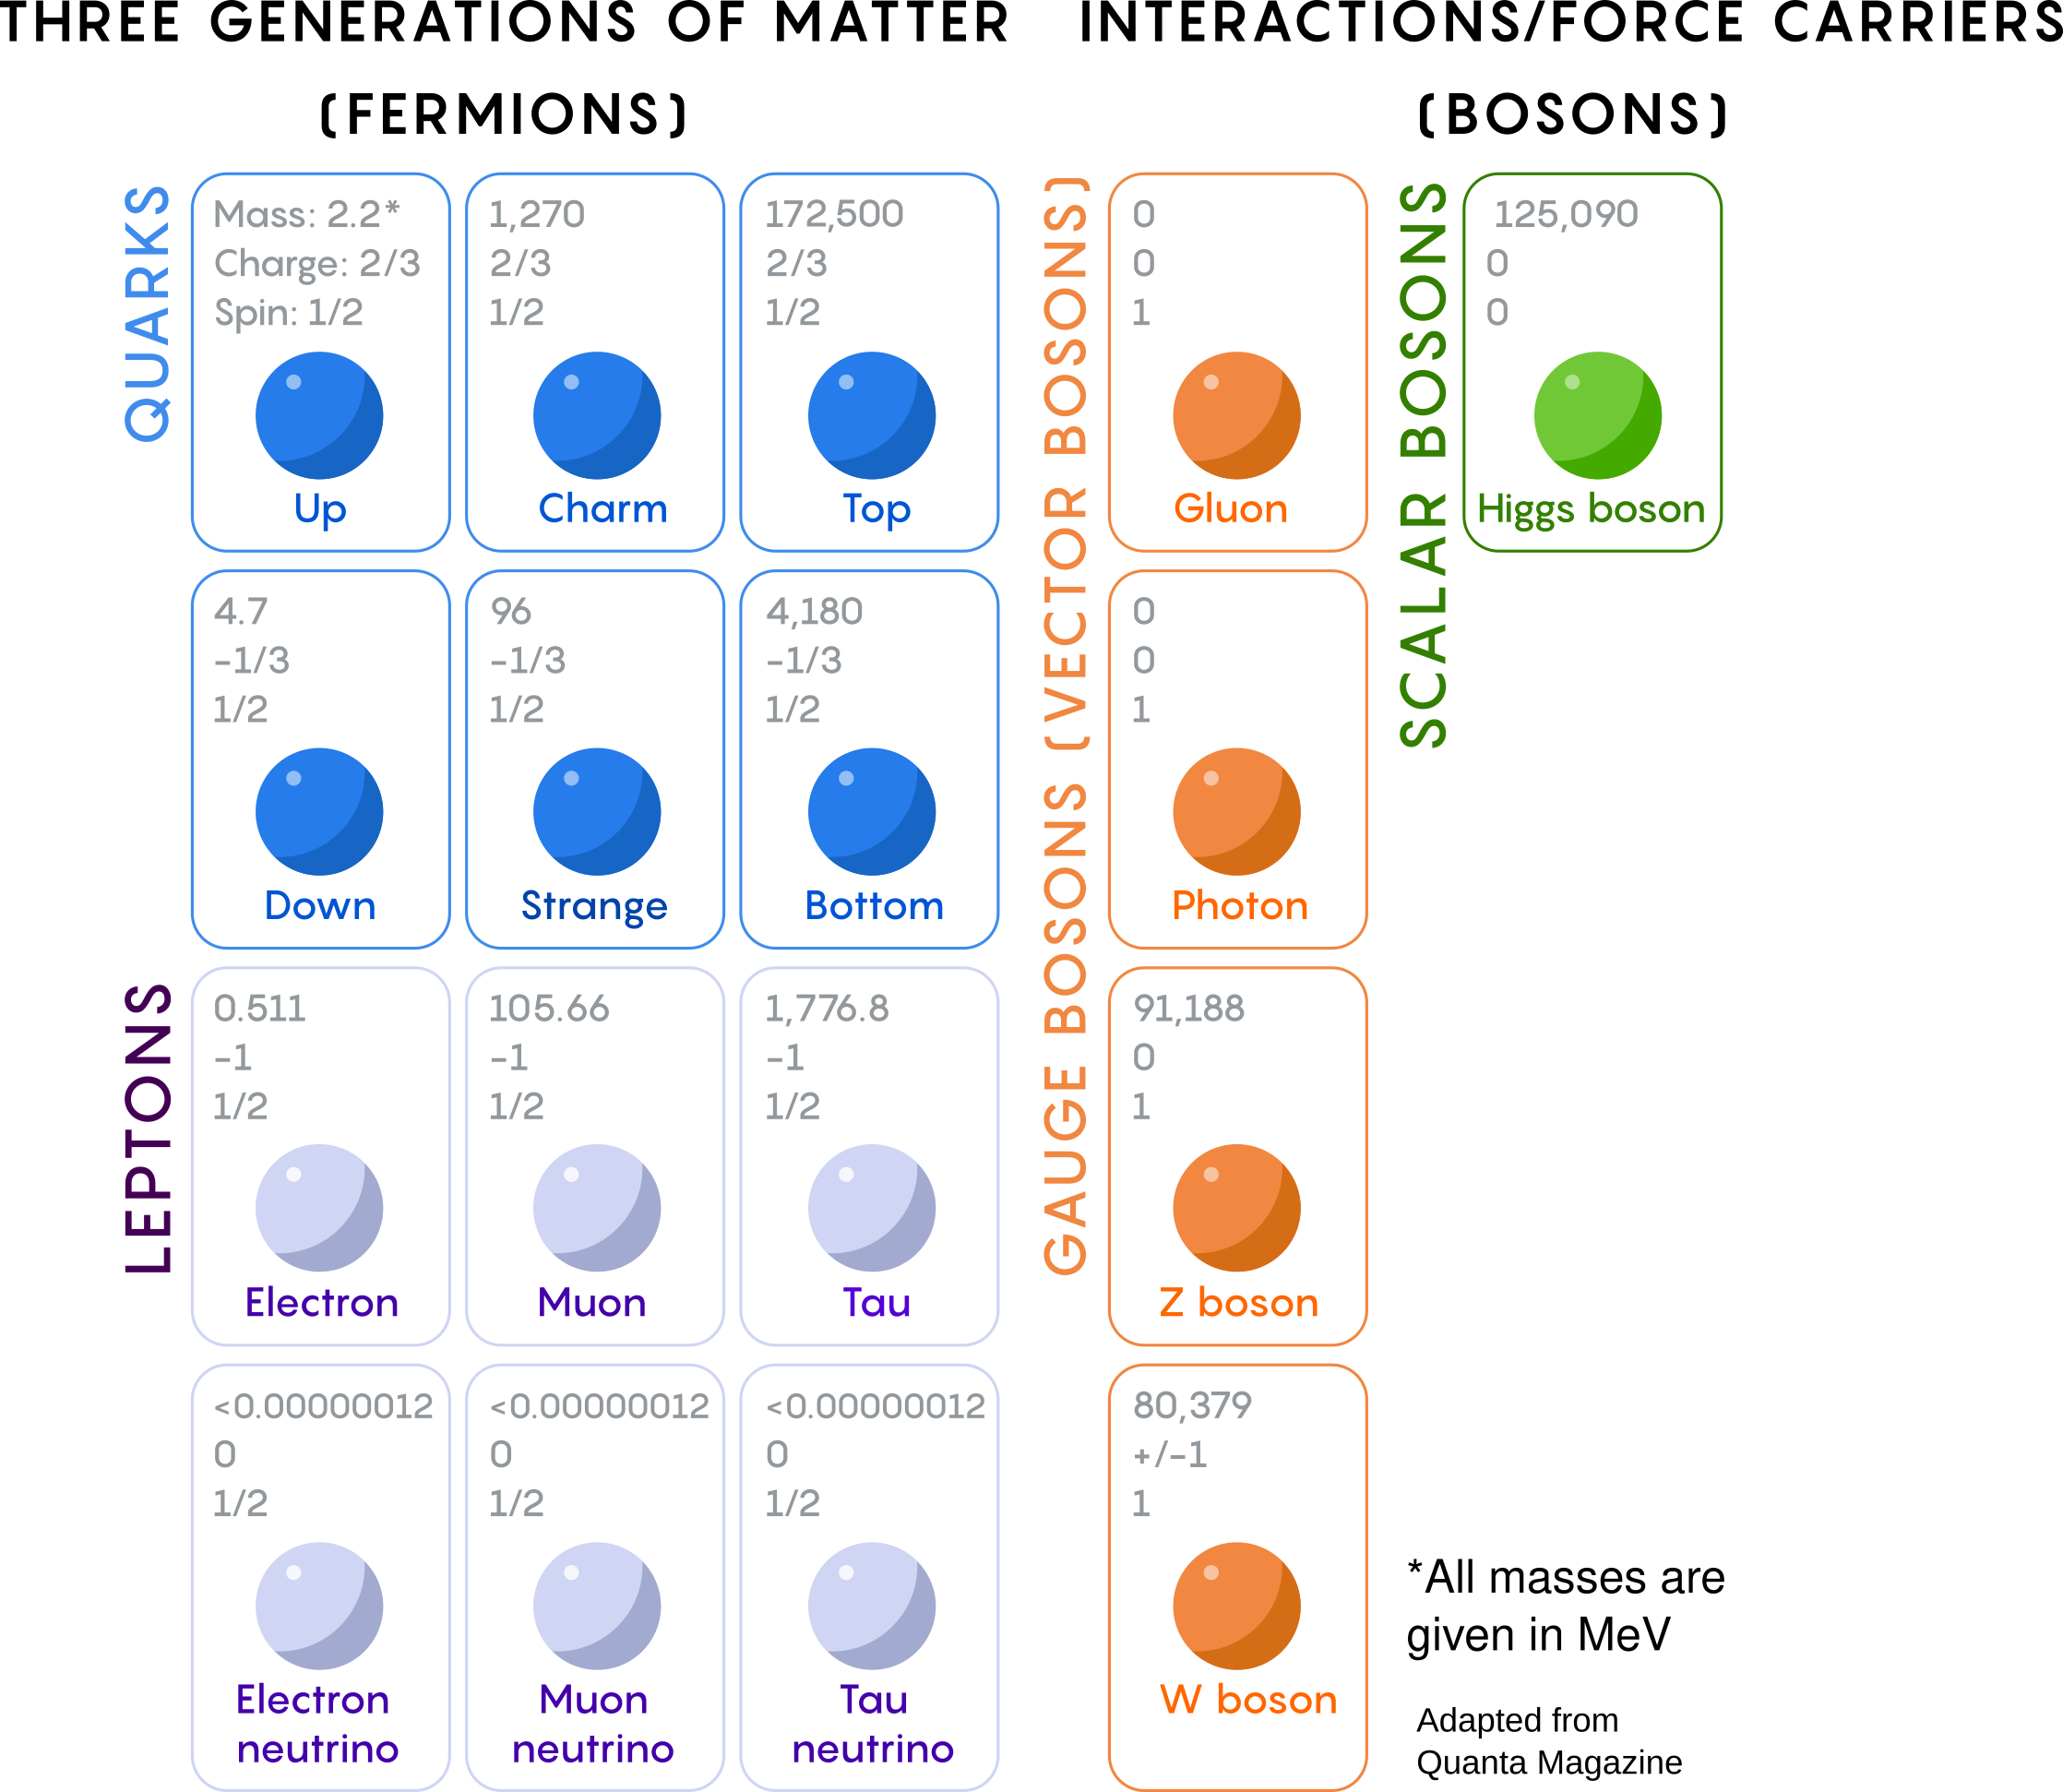
\includegraphics[width=0.60\textwidth]{figures/l1/intro/SM_qm_lm.png}
      \end{figure}
\end{frame}

\begin{frame}
  \frametitle{\bf The Higgs boson}
  \adjustbox{valign=c}{\begin{minipage}[t]{0.26\linewidth}
      \centering
      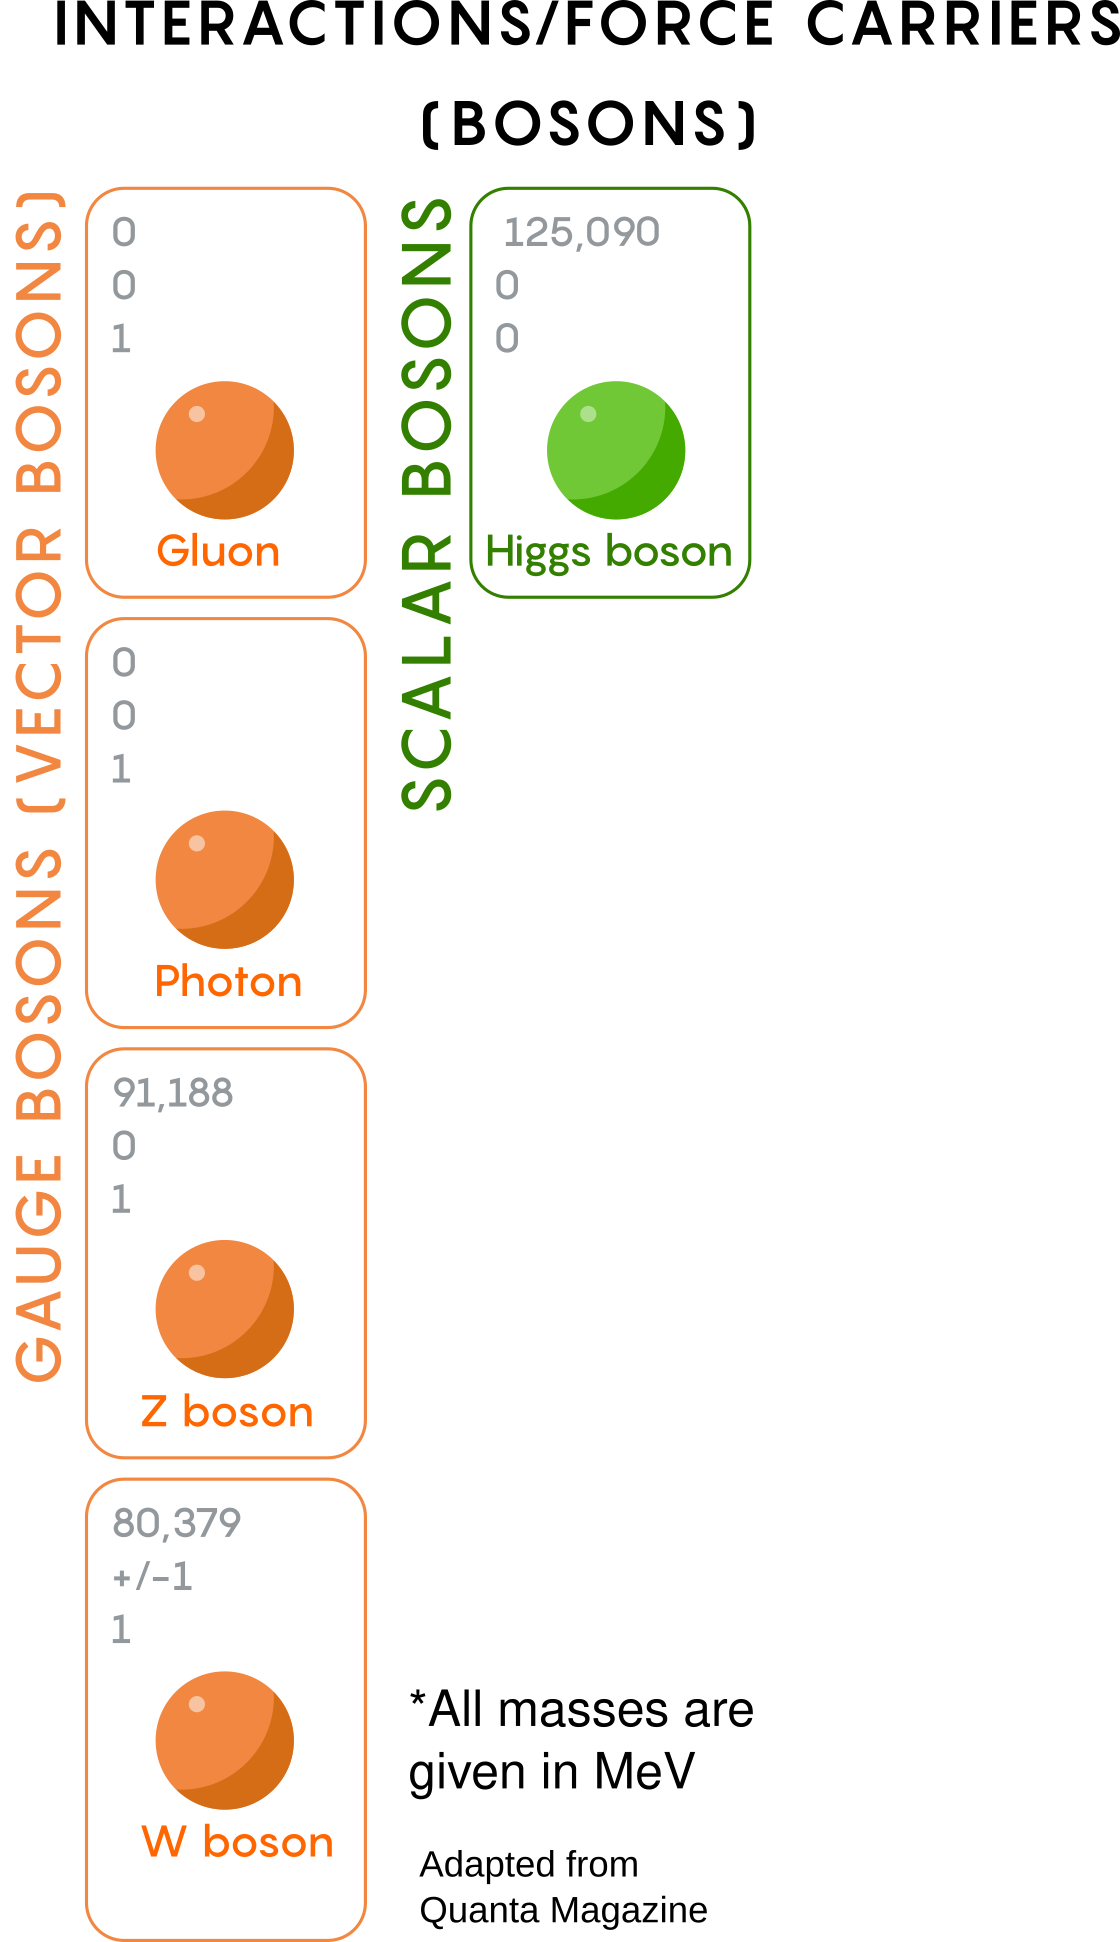
\includegraphics[width=0.98\textwidth]{figures/l1/intro/SM_qm_lm_bosons.png}
    \end{minipage}}\hfill
  \adjustbox{valign=c}{\begin{minipage}[t]{0.70\linewidth}
      \begin{itemize}
      \item 1964: R. Brout, F. Englert, P. Higgs:
        W, Z masses. 
      \item 2012: Higgs boson observation, ATLAS \& CMS
      \end{itemize}
      \hspace{0.1\textwidth}
      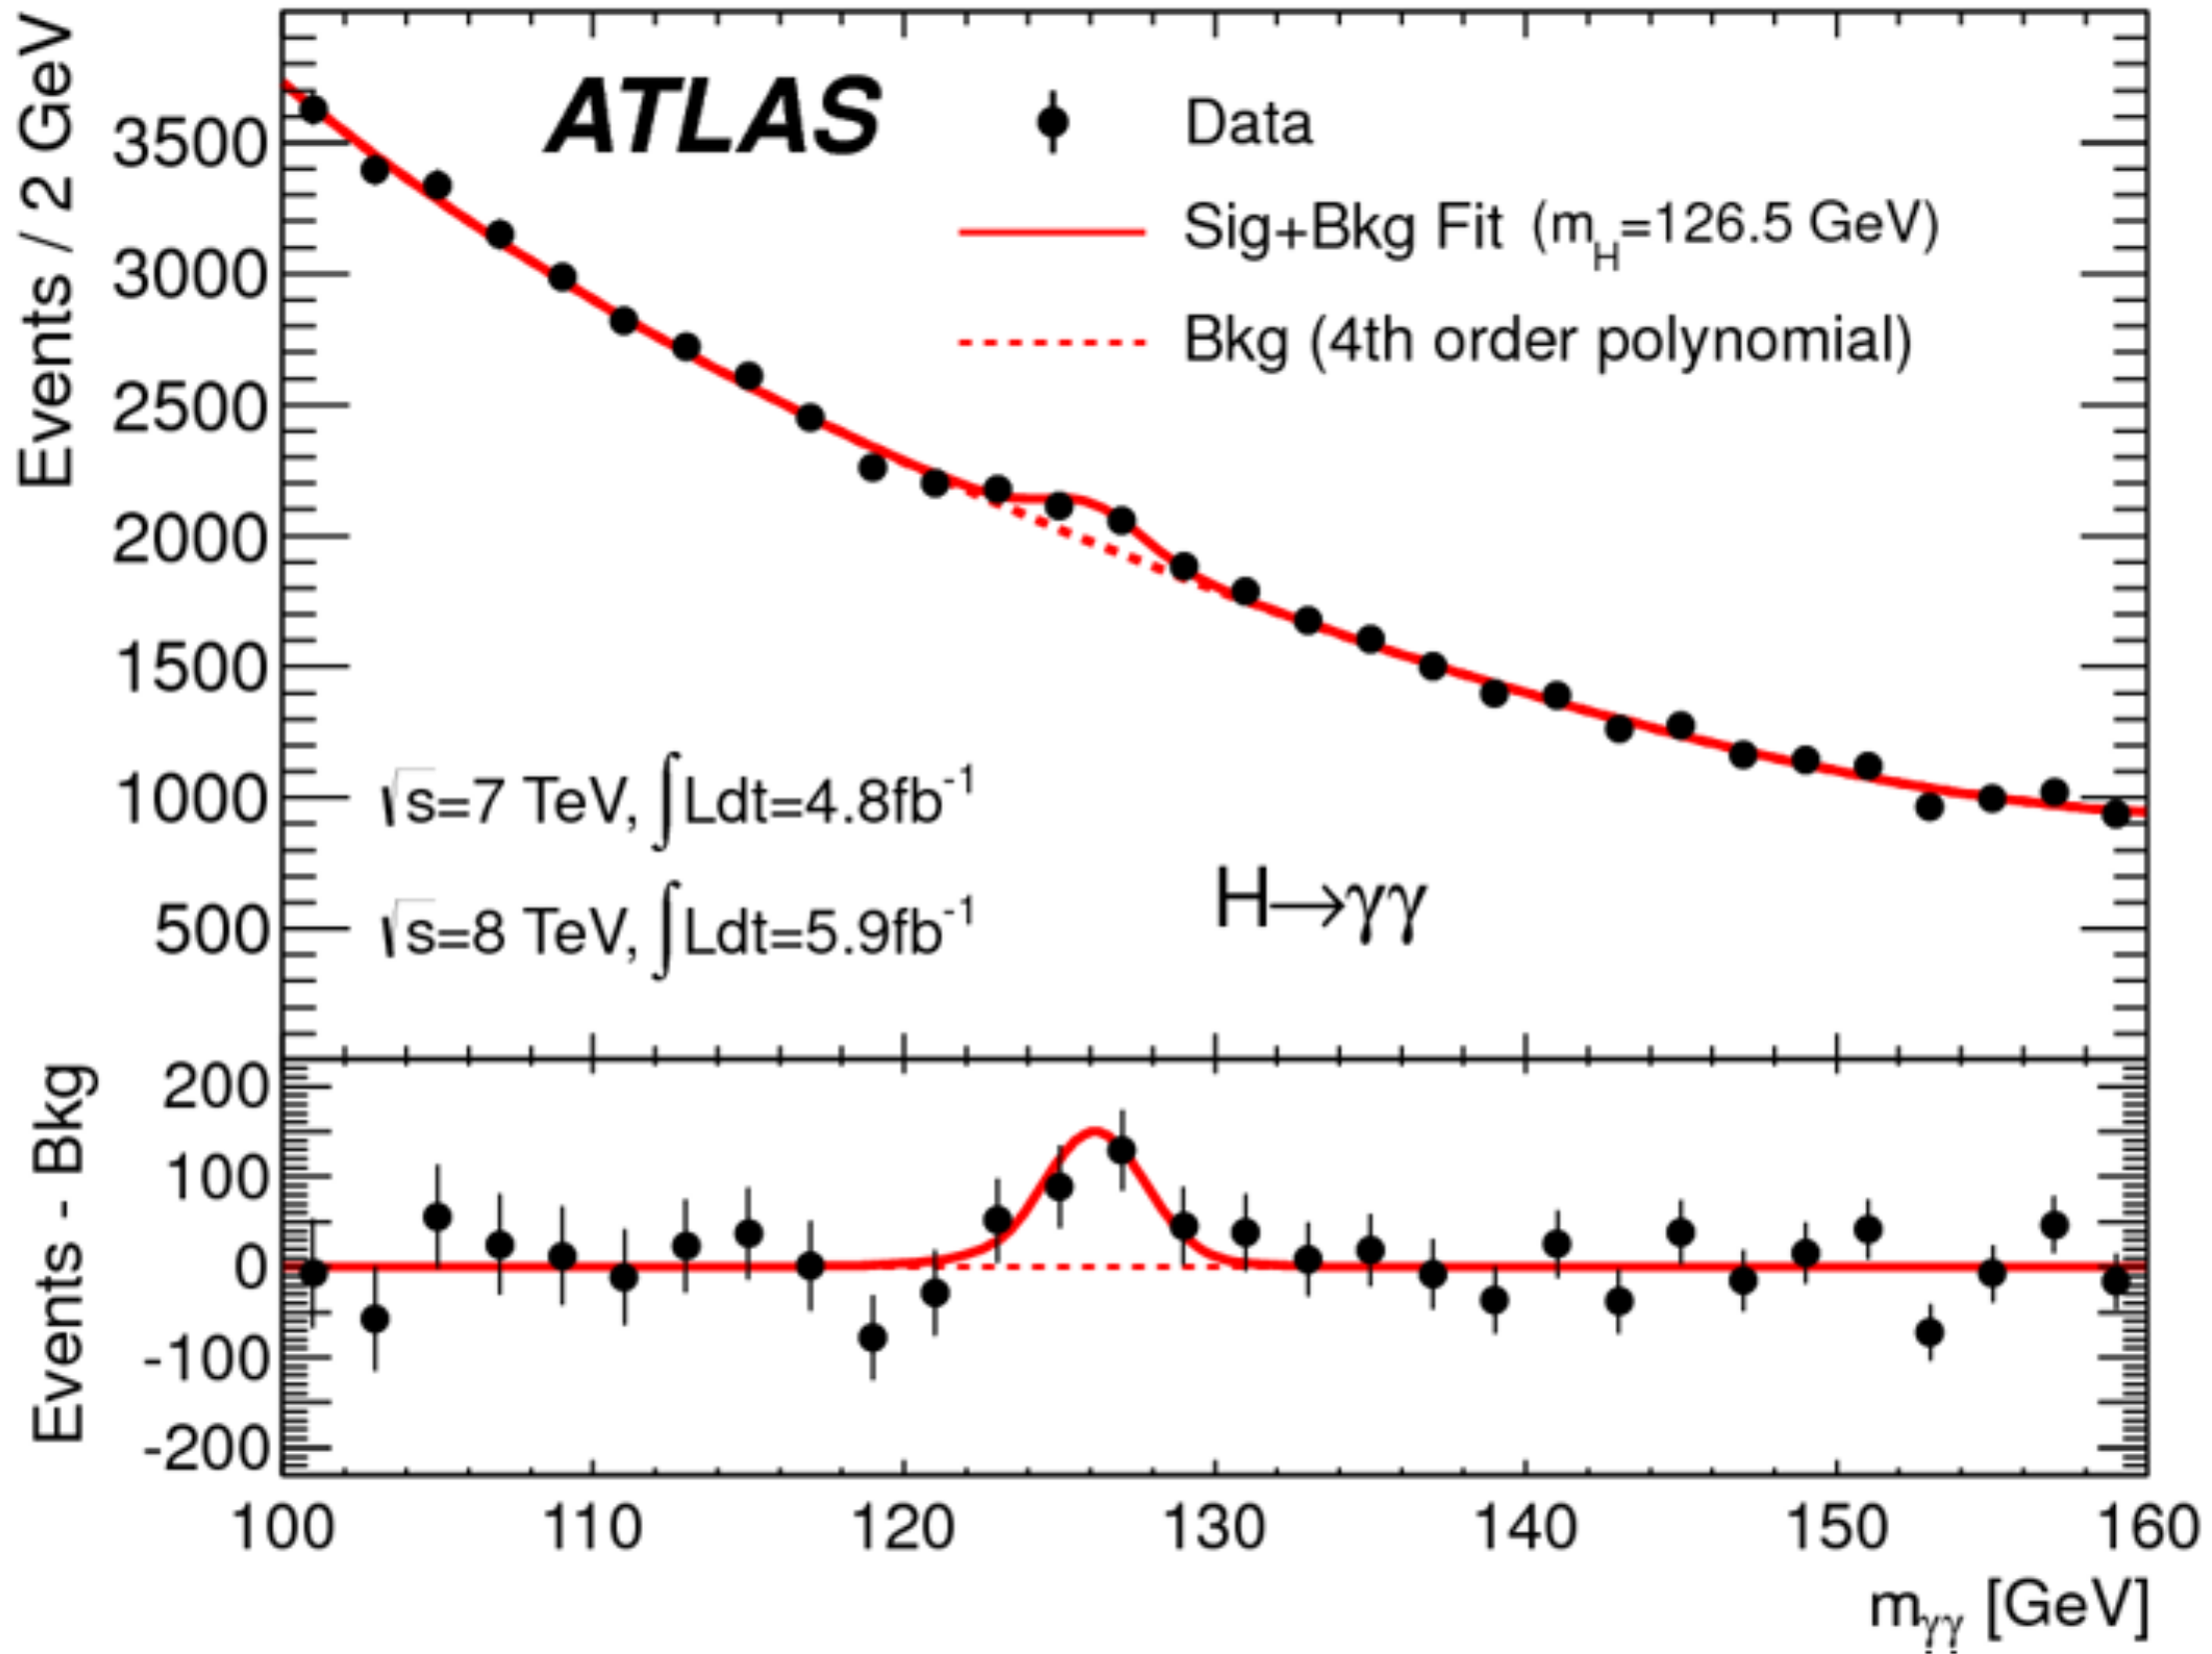
\includegraphics[width=0.6\textwidth]{figures/l1/intro/ATLAS_Higgs.png}
      \begin{itemize} 
      \item 2013: Nobel prize to F. Englert \& P. Higgs
      \end{itemize}      
    \end{minipage}}
\end{frame}


\end{document}


\begin{frame}
  \frametitle{\bf Higgs boson 10 years after discovery}
  \begin{itemize}
  \item Worlds best tH probe, by my PhD student Tom Carter.
  \item Key, innovative contributions by Edinburgh to all \textcolor{EDBDarkBlue}{\Hgamgamb{}} results. 
  \end{itemize}
  \vspace{-5pt}
  \begin{figure}
    \includegraphics[width=0.95\textwidth]{figures/intro_cf/nature/fig_03.pdf}  
  \end{figure}
  % Measurement is limited by statistical uncertainty on the number of signal
  % events.
  \vspace{-20pt}
  \blfootnote{\scriptsize{L. Mijovi\'c, ATLAS, Nature 607, pages 52-59 (2022)}} 
\end{frame}



\begin{frame}
  \frametitle{\bf Higgs boson 10 years after discovery}
  \begin{itemize}
  \item Higgs couplings $c$; $\kappa_i = c_i/c_i^{\mathrm{SM}}$.
  \end{itemize}
  \vspace{-5pt}
  \begin{figure}
    \includegraphics[width=0.49\textwidth]{figures/intro_cf/gamgam/fig_23.pdf}  
    \includegraphics[width=0.49\textwidth]{figures/intro_cf/nature/fig_05.pdf}  
  \end{figure}
  % Measurement is limited by statistical uncertainty on the number of signal
  % events.
  \vspace{-20pt}
  \blfootnote{\scriptsize{L. Mijovi\'c, ATLAS, accepted by JHEP (left), Nature
      607, pages 52-59 (2022) (right).}} 
\end{frame}





{
  \usebackgroundtemplate{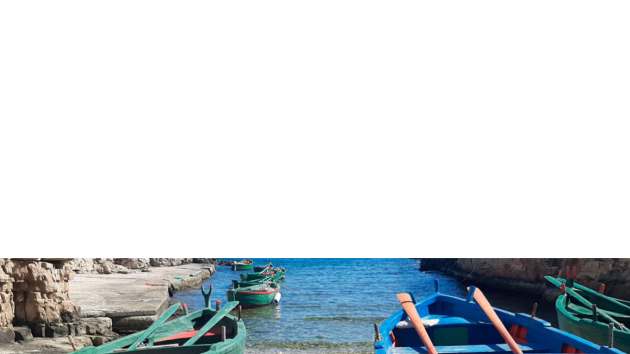
\includegraphics[width=\paperwidth]{background/template_169.pdf}}%
  \begin{frame}[plain]
  \begin{center}
    \setlength{\parskip}{0pt}
    {\huge\bf Key missing measurements in Higgs physics?}
  \end{center}    
  \adjustbox{valign=t}{\begin{minipage}[t]{0.24\linewidth} 
    \end{minipage}}
  \hfill
  \adjustbox{valign=t}{\begin{minipage}[t]{0.50\linewidth}
        \begin{center}
  \begin{itemize}
  \item {\huge \bf Higgs width}
  \item {\huge \bf Higgs potential}
    %\item[\textcolor{Gray}{\textbullet}] {\huge \bf \textcolor{Gray}{Higgs potential}}
    \end{itemize}
    \end{center}
  \end{minipage}}
\hfill
  \adjustbox{valign=t}{\begin{minipage}[t]{0.24\linewidth} 
    \end{minipage}}
\end{frame}
}

% -----------------------------------------------------------------------
% challenge
\begin{frame}[fragile]
  \frametitle{\bf Why Measure the Higgs Width?}
  \vspace{-10pt}  
  \begin{enumerate}
  \item[1)] Key properties of a fundamental particle: mass (m) and lifetime ($\tau$).\\
    Higgs boson: $\Delta{\mH}/\mH$: $\sim$ 1\permille, $\tau_\higgs$: not
    measured yet!\\   
    \textcolor{EDBBlue}{Measurement of the Higgs width (\gh{}) would determine
      Higgs lifetime: $\tau_\higgs = \hbar / \gh$.} 
   \adjustbox{valign=c}{\begin{minipage}[c]{0.5\linewidth}
    Width of a resonance:
    \begin{itemize}
    \item Heisenberg's uncertainty:
    $\Delta \mathrm{E}\Delta \mathrm{t} \geq \hbar/2$
  \item Einstein's relativity: $\mathrm{E} \sim \mathrm{mc}^2$
  \end{itemize}
 \end{minipage}}
 \adjustbox{valign=c}{\begin{minipage}[c]{0.35\linewidth}    
     \begin{figure}
       % \centering
       \vspace{5pt} 
     \includegraphics[width=0.95\textwidth,center]{figures/sketches/Breit-Wigner.pdf}
   \end{figure} 
 \end{minipage}}
\hfill
\vfill
\item[2)] Higgs couplings ($c$) are extracted from  cross-sections:
  $\sigma\,{\propto}\,c^2\,/\,\gh$.\\
  \textcolor{EDBBlue}{\gh{}: needed to reliably extract all
    Higgs couplings\\
    $\Rightarrow$ key for understanding of the origin of mass.}
\end{enumerate}

\end{frame}

\begin{frame}[fragile]
  \frametitle{\bf Higgs Width: the Challenge}
  \adjustbox{valign=c}{\begin{minipage}[c]{0.47\linewidth}
      \vspace{-10pt}
  \begin{itemize}
  \item Higgs boson is predicted to be\\
    very narrow: $\ghsm \sim 4.1\,\MeV$. 
%  \item $\ghsm/\mH \sim 0.03\cdot 10^{-3}$.
  \item Detector resolution: O(GeV).
  \end{itemize}
 \vspace{10pt}
  \adjustbox{valign=t}{\begin{minipage}[t]{0.49\linewidth}
      %\vspace{5pt}
       \includegraphics[width=0.99\textwidth,center]{figures/sketches/bw_sm_XLlet.png}
     \end{minipage}}
   \hfill
   \adjustbox{valign=t}{\begin{minipage}[t]{0.49\linewidth}
       %\vspace{5pt}
       \includegraphics[width=0.99\textwidth,center]{figures/sketches/bw_det_XLlet.png}
     \end{minipage}}
   \vfill
  \end{minipage}}
\adjustbox{valign=c}{\begin{minipage}[c]{0.48\linewidth}
    %\vspace{-15pt}
    \includegraphics[width=0.99\textwidth,center]{figures/slides_extra/1_challenge/cms_onshell_width.pdf}
  \end{minipage}}
%\vspace{-30pt}
% \begin{itemize}
%\vfill
\vspace{-20pt}
\begin{itemize}
\item Line-shape measurement [1]: %$\gh < 1.1$ \GeV;
$\gh \lesssim 300 \cdot \ghsm $.%262
\end{itemize}
\vfill
\begin{center}
%  \begin{tcolorbox}[colback=white,colframe=white,top=0pt,bottom=0pt,left=0pt,right=0pt,
%    text width=0.8\linewidth]
%    {\parbox{\textwidth}{
  \vspace{-5pt}
        \textcolor{EDBBlue}{Challenge: how would I measure the width?}
%      }}
%  \end{tcolorbox}
\end{center}
\vspace{-20pt}
\blfootnote{Figure [1]: CMS collaboration, \href{https://arxiv.org/abs/1706.09936}{JHEP {\bf 11} (2017) 047}.}
\end{frame}

\begin{frame}
  \frametitle{\bf My Novel Solution}
  \adjustbox{valign=t}{\begin{minipage}[t]{0.34\linewidth}
       \begin{itemize}
      \item \textcolor{EDBBlue}{Exploit QM interference.}
      \end{itemize}      
      \includegraphics[width=0.75\textwidth,center]{figures/gamma/dia/dia_ver.png}%
    \end{minipage}}
  \adjustbox{valign=t}{\begin{minipage}[t]{0.3\linewidth}
      \begin{itemize}
      \item \textcolor{EDBBlue}{Interference affects several $\gamma$ kinematic
          distributions [2]. }
      \item Example: $\gamma$ angle wrt. to the beam-line. 
      \end{itemize} 
    \end{minipage}}
  \adjustbox{valign=t}{\begin{minipage}[t]{0.34\linewidth}
      \begin{itemize}
      \item Size of the interference depends on \gh{}.
      \item \textcolor{EDBBlue}{Develop novel experimental techniques \& measure \gh{}.}
      \end{itemize} 
    \end{minipage}}
  \adjustbox{valign=c}{\begin{minipage}[t]{0.35\linewidth}
      \includegraphics[width=0.99\textwidth,center]{figures/sketches/double_slit.png}%
    \end{minipage}}
  \adjustbox{valign=c}{\begin{minipage}[t]{0.3\linewidth}
      \includegraphics[width=1.03\textwidth,center]{figures/gamma/kinematics/cos_th_CS.png}%
    \end{minipage}}
  \adjustbox{valign=c}{\begin{minipage}[t]{0.3\linewidth}
      \vspace{-12pt}
      \includegraphics[width=0.94\textwidth,center]{figures/gamma/summary/proj_gammas_annot.pdf}%}%
    \end{minipage}}
  \blfootnote{[2] Z. Liu, J. Campbell et al., \href{https://arxiv.org/abs/1704.08259}{Phys. Rev.
    Lett. {\bf 119}, 181801 (2017).}}
\end{frame}


\begin{frame}
  \frametitle{\bf My Novel Solution}
  \adjustbox{valign=t}{\begin{minipage}[t]{0.34\linewidth}
       \begin{itemize}
      \item \textcolor{EDBBlue}{Exploit QM interference.}
      \end{itemize}      
      \includegraphics[width=0.75\textwidth,center]{figures/gamma/dia/dia_ver.png}%
    \end{minipage}}
  \adjustbox{valign=t}{\begin{minipage}[t]{0.3\linewidth}
      \begin{itemize}
      \item \textcolor{EDBBlue}{Interference affects several $\gamma$ kinematic
          distributions [2]. }
      \item Example: $\gamma$ angle wrt. to the beam-line. 
      \end{itemize} 
    \end{minipage}}
  \adjustbox{valign=t}{\begin{minipage}[t]{0.34\linewidth}
      \begin{itemize}
      \item Size of the interference depends on \gh{}.
      \item \textcolor{EDBBlue}{Develop novel experimental techniques \& measure \gh{}.}
      \end{itemize} 
    \end{minipage}}
  \adjustbox{valign=c}{\begin{minipage}[t]{0.35\linewidth}
      \includegraphics[width=0.99\textwidth,center]{figures/sketches/double_slit.png}%
    \end{minipage}}
  \adjustbox{valign=c}{\begin{minipage}[t]{0.3\linewidth}
      \includegraphics[width=1.03\textwidth,center]{figures/gamma/kinematics/cos_th_CS.png}%
    \end{minipage}}
  \adjustbox{valign=c}{\begin{minipage}[t]{0.3\linewidth}
      \vspace{-12pt}
      \includegraphics[width=0.94\textwidth,center]{figures/gamma/summary/proj_gammas_annot_p2.pdf}%}%
    \end{minipage}}
  \blfootnote{[2] Z. Liu, J. Campbell et al., \href{https://arxiv.org/abs/1704.08259}{Phys. Rev.
    Lett. {\bf 119}, 181801 (2017).}}
\end{frame}

% -----------------------------------------------------------------------
% what's special about my method?
\begin{frame}
  \frametitle{\bf Why is My Solution Unique?}
  \begin{minipage}[t][0.1\textheight]{\linewidth}
    \vspace{5pt}
    Because it would probe \gh{} with \textcolor{EDBRed}{high sensitivity} in \textcolor{EDBBlue}{On-Shell} events.
  \end{minipage}
  \vfill
   \begin{minipage}[t][0.7\textheight]{\linewidth}
    \vspace{10pt}
    \textcolor{Gray}{State-of-the-art techniques: line-shape measurement,
      mass shift in \Hgamgam{},}\\ off-shell interference in
    ${\Higgs^*}{\rightarrow}\mathrm{VV}$ events, \textcolor{Gray}{\tauh{}
      from secondary vertex displacement $\ldots$}
  \end{minipage}
\end{frame}
  
\begin{frame}
  \frametitle{\bf Why is My Solution Unique?}
  \addtocounter{framenumber}{-1}
  \begin{minipage}[t][0.1\textheight]{\linewidth}
    \vspace{5pt}
    Because it would probe \gh{} with \textcolor{EDBRed}{high sensitivity} in \textcolor{EDBBlue}{On-Shell} events.
  \end{minipage}% end 0.1\textheight page
  \vfill
  \begin{minipage}[t][0.7\textheight]{\linewidth}
    \vspace{10pt}
    \adjustbox{valign=t}{\begin{minipage}[t]{0.45\linewidth}
        \textcolor{orange}{Off-shell} interference:
        \vspace{5pt}
        \begin{itemize}
        \item \textcolor{EDBRed}{1-$\sigma$ sensitivity [3]: $\gh{}/\ghsm{} \sim
            0.8$.}
        \end{itemize}
        \begin{itemize}
        \item Sensitivity: far off-shell tail.
        \end{itemize}
        \begin{itemize} 
        \item \textcolor{orange}{Assumption: $\mu_{\mathrm{off}}/{\mu_{\mathrm{on}}} = 1.$} 
        \end{itemize}
        \begin{itemize}
        \item Not valid in most classes of BSM\\
        models. Eg. [4]: extra scalar - MSSM $\tilde{\mathrm{t}}$, EFT $\ldots$
      \end{itemize}
    \end{minipage}}
  \adjustbox{valign=t}{\begin{minipage}[t]{0.45\linewidth} 
      \includegraphics[width=0.95\textwidth,center]{figures/sketches/Breit-Wigner_offshell_bad_annot.pdf}%
    \end{minipage}}
\end{minipage}% end 0.8\textheight page
\vspace{-20pt}
  \blfootnote{[3] ATLAS,
    \href{https://indico.cern.ch/event/1086716/contributions/5058702/attachments/2543934/4380724/Higgs2022_mveen_v3.pdf}{Higgs
      2022}. $\gh{}/\ghsm{} \sim 0.98$ reached by CMS, \href{https://arxiv.org/abs/2202.06923}{Nature Phys. (2022)}. [4]
    \href{https://arxiv.org/abs/1410.5440}{C. Englert et. al, JHEP {\bf 05} (2015) 145}.}  
\end{frame}
%https://www.nature.com/articles/s41567-022-01682-0 [0.6,8.1]

\begin{frame}
  
  \frametitle{\bf Why is My Solution Unique?}
  \addtocounter{framenumber}{-1}
  \begin{minipage}[t][0.1\textheight]{\linewidth}
    \vspace{5pt}
    Because it would probe \gh{} with \textcolor{EDBRed}{high sensitivity} in \textcolor{EDBBlue}{On-Shell} events.
  \end{minipage}% end 0.1\textheight page
  \vfill
  \begin{minipage}[t][0.7\textheight]{\linewidth}
    \vspace{10pt}
    \adjustbox{valign=t}{\begin{minipage}[t]{0.45\linewidth}
        My Solution:
          \vspace{5pt}
        \begin{itemize}      
        \item \textcolor{EDBBlue}{On-Shell events.}
        \end{itemize}
        \vspace{4pt}
        \begin{itemize}  
          \item \textcolor{EDBRed}{1-$\sigma$ sensitivity: $\gh{}/\ghsm{} \sim 1$.}
          \end{itemize}
          \vspace{4pt}
          \begin{itemize}   
          \item \textcolor{orange}{No assumption: $\mu_{\mathrm{off}}/\mu_{\mathrm{on}} = 1.$} 
          \end{itemize} 
    \end{minipage}}
  \adjustbox{valign=t}{\begin{minipage}[t]{0.45\linewidth} 
      \includegraphics[width=0.95\textwidth,center]{figures/sketches/Breit-Wigner_onshell_good.pdf}%
    \end{minipage}}
\end{minipage}% end 0.8\textheight page
\vspace{-20pt}
 \blfootnote{}  
\end{frame}
%https://www.nature.com/articles/s41567-022-01682-0 [0.6,8.1]


%%% ------------------------------------------------------------------------------
%%% WP2: gh measurement frame 
%%  
%%  \begin{frame}
%%    \frametitle{\bf Measurement of \gh{}}
%%    %Strategy: measure \gh{} using on-shell interference in \Hgamgam{} events
%%    \includegraphics[width=0.7\textwidth,center]{figures/gamma/dia/dia_hor.png}%
%%    \vfill
%%    \vspace{2pt}
%%    \adjustbox{valign=c}{\begin{minipage}[t]{0.325\linewidth} 
%%      \includegraphics[width=0.99\textwidth]{figures/gamma/kinematics/feature_rank.png}%
%%    \end{minipage}}
%%    \adjustbox{valign=c}{\begin{minipage}[t]{0.325\linewidth} 
%%      \includegraphics[width=0.99\textwidth]{figures/gamma/kinematics/bdt_disc.pdf}%
%%    \end{minipage}}
%%  \adjustbox{valign=c}{\begin{minipage}[t]{0.325\linewidth} 
%%      \includegraphics[width=0.99\textwidth]{figures/gamma/kinematics/cos_th_CS.png}%
%%    \end{minipage}}
%%  \vfill
%%  \begin{itemize}
%%  \item Catch: interference effects are largest in events with low-\pt{} $\gamma$.
%%  \item Currently not triggered by ATLAS, due to high background rates.
%%  \item \textcolor{EDBBlue}{Events most sensitive to \gh{} are lost to experimental analyses!}
%%  \end{itemize}
%%  \end{frame}
%% 
% end of WP2: gh measurement
% ------------------------------------------------------------------------------


\begin{frame}[fragile]
  \frametitle{\bf The Catch: Trigger}
  \begin{itemize}
  \item {\bf Detector: snap-shot of collision.}
  \item {\bf Trigger: reduces the rate from 40 MHz to 1kHz.}
  \end{itemize}  
  \begin{figure}
    \includegraphics[height=0.40\textheight]{figures/intro_cf/lhc_coll.png}
    \includegraphics[height=0.40\textheight]{figures/camera.png}
  \end{figure}
  \begin{itemize}
  \item {\bf No trigger for \gamgamb{} events sensitive to \gh{}.}
  \item {\bf These events are forever lost to experimental analyses!}
  \end{itemize}  
\end{frame}


% ------------------------------------------------------------------------------
% WP1: trigger 
    
  \begin{frame}
    \frametitle{\bf New \gamgamb{} triggers}
    \vspace{-12pt}
    \begin{itemize}
    \item Develop new triggers harnessing upgrade of ATLAS trigger. 
%    \item Ugrade: EM calorimeter readout \& topological
%      hardware trigger.
 %   \item Proposal: develop new triggers harnessing the upgrade. Capture 
 %     events sensitive to \gh{} at sufficiently low rates for
 %     inclusion in the  ATLAS trigger menu. 
    \end{itemize}
    \vfill 
    \adjustbox{valign=c}{\begin{minipage}[t]{0.49\linewidth} 
        \begin{figure}
          \includegraphics[width=0.99\textwidth]{figures/gamma/kinematics/cos_th_CS.png}
        \end{figure} 
      \end{minipage}}
    \adjustbox{valign=c}{\begin{minipage}[t]{0.49\linewidth}  
        \includegraphics[width=.95\textwidth]{figures/gamma/trig/trig.png}
      \end{minipage}}
%    \begin{itemize} 
%    \item $\sim$14x higher sensitivity to \gh{}, compared to baseline ATLAS trigger.
    New triggers: key to reaching ground-breaking sensitivity:
    \begin{itemize}
    \item \textcolor{EDBRed}{LHC: 1-$\sigma$ sensitivity: $\gh{}/\ghsm{} \sim 1$.}
    \item \textcolor{EDBRed}{HL-LHC: possibly $\gh{}/\ghsm{} <$ 5\%?}   
    \end{itemize}

  \end{frame}
% -----------------------------------------------------------------------

\begin{frame}
  \frametitle{\bf What if I Measure a Deviation from SM?}
  \begin{itemize}
  \item New particles coupling to the Higgs boson?
  \item Scalar (S) explaining the matter-antimatter asymmetry of the
    Universe [3]?
  \end{itemize}   
  \begin{figure}
    \includegraphics[height=0.58\textheight]{figures/cf_2020/exciting_intro/Z_3gen.png}%
    \includegraphics[height=0.58\textheight]{figures/gamma/bsm/bsm_carena_ewpt_fut.png}%
  \end{figure}
  \vspace{-10pt}
  \begin{itemize}
  \item {\bf Plan: harness Higgs centre to organize theory-experiment workshops.}
  \end{itemize}
  \vspace{-10pt}  
  \blfootnote{[3] Carena et al., Electroweak phase transition with spontaneous
    Z2-breaking, \href{https://arxiv.org/abs/1911.10206}{JHEP 08 (2020) 107}.}
\end{frame}

%%\begin{frame}
%%  \frametitle{\bf What if I Measure a Deviation from SM?}
%%  \begin{itemize}
%%  \item New particles coupling to the Higgs boson?
%%  \item Scalar (S) explaining the matter-antimatter asymmetry of the
%%    Universe [3]?
%%  \end{itemize}   
%%  \begin{figure}
%%    \includegraphics[height=0.58\textheight]{figures/cf_2020/exciting_intro/Z_3gen.png}%
%%    \includegraphics[height=0.58\textheight]{figures/gamma/bsm/bsm_carena_ewpt.png}%
%%  \end{figure}
%%  \vspace{-10pt}
%%  \begin{itemize}
%%  \item {\bf Plan: harness Higgs centre to organize theory-experiment workshops.}
%%  \end{itemize}
%%  \vspace{-10pt}  
%%  \blfootnote{[3] Carena et al., Electroweak phase transition with spontaneous
%%    Z2-breaking, \href{https://arxiv.org/abs/1911.10206}{JHEP 08 (2020) 107}.}
%%\end{frame}

\begin{frame}
  \frametitle{\bf What if I Don't Measure a Deviation?}
  \begin{itemize}
  \item {\bf Remember: $\tau_\higgs$ and all Higgs couplings!} 
  \end{itemize} 
   \begin{figure}
     \includegraphics[width=.7\textwidth]{figures/snowmass/HiggsPrecisionSummary.pdf}
   \end{figure}
   \vspace{-15pt}
   \blfootnote{Figure: Muon Collider Forum Report, Snowmass 2021, \href{https://arxiv.org/abs/2209.01318}{arXiv:2209.01318 (2022)}}.
\end{frame}

%--------------------------------------------

{
\usebackgroundtemplate{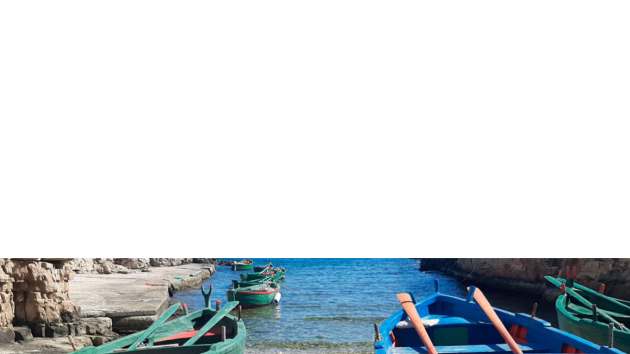
\includegraphics[width=\paperwidth]{background/template_169.pdf}}%
\begin{frame}[plain]  
  \adjustbox{valign=t}{\begin{minipage}[t]{0.24\linewidth} 
    \end{minipage}}
  \hfill
  \adjustbox{valign=t}{\begin{minipage}[t]{0.50\linewidth}     
  \begin{center}
    \setlength{\parskip}{0pt}
    \vspace{10pt}
    {\Huge\bf Synergies}
  \end{center}
  \begin{itemize}
    \item {\Large \bf Machine Learning}
    \item {\Large \bf Particle Physics Theory}
    \item {\Large \bf Outreach}
    \end{itemize}
  \end{minipage}}
\hfill
  \adjustbox{valign=t}{\begin{minipage}[t]{0.24\linewidth} 
    \end{minipage}}
\end{frame}
}

{
  \usebackgroundtemplate{\includegraphics[width=\paperwidth]{figures/chanc/synergy/lm_ml_projects.pdf}}%
%\begin{frame}[noframenumbering,plain]
\begin{frame}[fragile]
  \frametitle{\bf Machine learning: track record}
  \vspace{-2pt}
  \adjustbox{valign=t}{\begin{minipage}[t][0.42\textheight]{\linewidth}
      \adjustbox{valign=t}{\begin{minipage}[t]{0.47\linewidth} 
         {\bf First ML track reconstruction}
          \vfill
      \end{minipage}}
    \hfill
      \adjustbox{valign=t}{\begin{minipage}[t]{0.52\linewidth} 
          {\bf Optimal \ttHb{} classification with ANNs}
          \vfill
        \end{minipage}}
    \end{minipage}}
  \vfill
  \adjustbox{valign=t}{\begin{minipage}[t][0.45\textheight]{\linewidth} 
      \adjustbox{valign=t}{\begin{minipage}[t]{0.47\linewidth} 
           {\bf Best tH,\Hgamgamb{} classification}
            \vfill
        \end{minipage}}   
    \hfill
      \adjustbox{valign=t}{\begin{minipage}[t]{0.52\linewidth} 
          {\bf ML-generated synthetic data for \Hgamgamb{}}
          \vfill
        \end{minipage}}
    \end{minipage}}
  \vspace{-26pt}
  \blfootnote{Work by: Ewan Miller, Keira Farmer, Jenifer Curran, Tom Carter, Dr. Matt Heath.}
\end{frame}
}


{
\usebackgroundtemplate{\includegraphics[width=\paperwidth]{figures/chanc/synergy/lm_ml.pdf}}%
%\begin{frame}[noframenumbering,plain]
\begin{frame}
\frametitle{\bf Machine learning: network}
% $\sim$50 experts from ML industry and physics fields. We have the mandate to
% identify key classes of problems which affect our work, and potential
% solutions, and publish a \textcolor{EDBBlue}{white paper in Nature Reviews
% Physics}.
  \adjustbox{valign=t}{\begin{minipage}[t][0.38\textheight]{\linewidth}
      \vspace{10pt}
      \adjustbox{valign=t}{\begin{minipage}[t]{0.52\linewidth} 
          \textcolor{White}{\bf \large Nature Reviews Physics Whitepaper}
          \begin{itemize}
            \item[\textcolor{white}{\textbullet}] \textcolor{White}{\bf $\sim$50
                invited ML experts}
            \item[\textcolor{white}{\textbullet}] \textcolor{White}{\bf Physics
                \& industry}
            \item[\textcolor{white}{\textbullet}] \textcolor{White}{\bf ID key classes of problems \&\\  potential solutions}
          \end{itemize}
      \end{minipage}}
    \hfill
      \adjustbox{valign=t}{\begin{minipage}[t]{0.47\linewidth} 
          \textcolor{White}{\bf \large Alan Turing Institute Fellowship}
          \begin{itemize}
            \item[\textcolor{white}{\textbullet}] \textcolor{White}{\bf
                Networking:\,bioscience,\,informatics.}
            %\item[\textcolor{white}{\textbullet}] \textcolor{White}{\bf Turing enrichment for PhD-s.}
          \end{itemize}
        \end{minipage}}
    \end{minipage}}
  \vfill
  \adjustbox{valign=t}{\begin{minipage}[t][0.38\textheight]{\linewidth}
      \vspace{-5pt}
      \adjustbox{valign=t}{\begin{minipage}[t]{0.52\linewidth} 
           \textcolor{White}{\bf \large Clinical AI Turing Group}
           \begin{itemize}
            \item[\textcolor{white}{\textbullet}] \textcolor{White}{\bf ML
                experts from academia,\\ health professionals, industry.} 
            \item[\textcolor{white}{\textbullet}] \textcolor{White}{\bf How to
                use AI for clinical benefits?}
            \end{itemize}
            \vfill
        \end{minipage}}   
    \hfill
      \adjustbox{valign=t}{\begin{minipage}[t]{0.49\linewidth} 
          \textcolor{White}{\bf \large Invited\,Lecturer}
           \begin{itemize}
            \item[\textcolor{white}{\textbullet}] \textcolor{White}{\bf \,DeepLearn\,2023\,\ldots}
            \end{itemize}
          \vfill
        \end{minipage}}
      \vfill
      \vspace{-10pt}
        {\bf Plan: win funding for interdisciplinary ML research, increase impact.}
    \end{minipage}}
\end{frame}
}

\begin{frame}[fragile]
  \frametitle{\bf Particle Physics Theory}
  \adjustbox{valign=t}{\begin{minipage}[t]{0.61\linewidth}
       \begin{figure}
         \includegraphics[width=0.9\textwidth]{figures/chanc/synergy/hej/hej_mjj.png}%
        \end{figure}            
      \end{minipage}}
    \hfill
    \adjustbox{valign=t}{\begin{minipage}[t]{0.30\linewidth}
        \textcolor{Orange}{\bf HEJ resummation:}
        \begin{figure}
           \includegraphics[width=0.7\textwidth]{figures/chanc/synergy/hej/hej.png}%
         \end{figure}
         {\bf Vector Boson Fusion:
        \begin{figure}
           \includegraphics[width=0.7\textwidth]{figures/chanc/synergy/VectorBosonFusion.png}%
         \end{figure}         
       \end{minipage}}
     \vspace{5pt}
     
     {\bf Plan: simulate HEJ+2jet predictions for ATLAS Higgs analyses.}
%     {\bf More broadly: collaborate with Theory on precision calculations \& parton distribution functions.}
 \blfootnote{Image credit: J.
   Paltrinieri,\href{https://indico.cern.ch/event/1186109/contributions/5063635/attachments/2531794/4356235/HEJ_VBF_JP.pdf}{\underline{LHC
       Higgs XS WG meeting}}.}    
\end{frame}

\begin{frame}[fragile]
  \frametitle{\bf Outreach}
  \adjustbox{valign=t}{\begin{minipage}[t][0.38\textheight]{\linewidth}
      \adjustbox{valign=t}{\begin{minipage}[c]{0.78\linewidth}
          \vspace{15pt}
          \begin{itemize}
          \item Funding: school's outreach funds \& Higgs centre.
          \item  \textcolor{EDBDarkBlue}{\bf Hands-on}: data released to public through CERN opendata. 
          \item  \textcolor{EDBDarkBlue}{\bf CERN Masterclass}: reaches $\sim$ 10k high-school students/year.
          \end{itemize}           
      \end{minipage}}
    \hfill
    \adjustbox{valign=t}{\begin{minipage}[c]{0.2\linewidth}
        \hfill
          \includegraphics[height=0.3\textheight]{figures/chanc/synergy/logos_out.pdf}%
        \end{minipage}}      
    \end{minipage}}
  \adjustbox{valign=t}{\begin{minipage}[t][0.45\textheight]{\linewidth}
      \includegraphics[height=0.4\textheight]{figures/chanc/synergy/du/higgs.png}%
      \includegraphics[height=0.4\textheight]{figures/chanc/synergy/du/comp1.png}%
      \includegraphics[height=0.4\textheight]{figures/chanc/synergy/du/comp2.png}%      
    \end{minipage}}
  \vfill
  \vspace{-30pt}
  \blfootnote{Photos courtesy of Higgs centre (I. Foidl) \& Radboud University, \href{ https://www.linkedin.com/company/studievereniging-leonardo-da-vinci/?originalSubdomain=nl}{\underline{ study association Leonardo Da Vinci}}}
\end{frame}


{
\usebackgroundtemplate{\includegraphics[width=\paperwidth]{figures/chanc/synergy/out_results.pdf}}%
\begin{frame}[fragile]
  \frametitle{\bf Outreach}
  \adjustbox{valign=t}{\begin{minipage}[t][0.45\textheight]{\linewidth}
      \begin{itemize}
      \item Explain particle signatures in the detector.
      \item Groups classify ATLAS event displays.
      \item Combine results of all groups.
      \item \textcolor{EDBDarkBlue}{\bf Success: Z boson (re-)discovered!}
      \item \textcolor{Violet}{\bf Quiz: mental.}
      \end{itemize}       
    \end{minipage}}
  \vfill
  \adjustbox{valign=t}{\begin{minipage}[t][0.45\textheight]{\linewidth} 
 \end{minipage}}
\end{frame}
}

\begin{frame}[fragile]
  \frametitle{\bf Outreach: plans}
  \adjustbox{valign=t}{\begin{minipage}[t]{0.63\linewidth}
      \vspace{10pt}
      \begin{itemize}
      \item Manual event classification:
        \begin{itemize}
        \item Z-boson: \textcolor{ForestGreen}{${\bm \checkmark}$}  
        \item Higgs boson: \textcolor{EDBRed}{$\text{{\bf \sffamily X}}$}  
          \end{itemize}
      \item \textcolor{EDBRed}{\bf No classroom exercise to discover the Higgs.}
      \end{itemize}
      \vspace{25pt}
      \vfill
      \textcolor{EDBRed}{\bf Plan: design it.}
      \begin{itemize}  
      \item CERN OpenData: 10-x events for Higgs discovery.
      \item Design simple ML classification.
      \item Run it over OpenData events.  
%      \item Pilot study: expect rediscovery.
      \end{itemize}
      \textcolor{EDBRed}{\bf Big challenge, would be huge break-through.}
    \end{minipage}}
  \adjustbox{valign=t}{\begin{minipage}[t]{0.35\linewidth}
      \begin{figure}
        \includegraphics[width=1.0\textwidth]{figures/chanc/synergy/bdt_disc_exp.pdf}%
      \end{figure}
      \vspace{-27pt}
       \begin{figure}
         \includegraphics[width=1.0\textwidth]{figures/chanc/synergy/myy_exp.pdf}%
        \end{figure} 
      \end{minipage}}
    \vspace{-15pt}
    \blfootnote{Work with James Cranmer, \href{https://github.com/FindTheHiggs/About}{https://github.com/FindTheHiggs}.}
\end{frame}

{
\usebackgroundtemplate{\includegraphics[width=\paperwidth]{background/template_169.pdf}}%
\begin{frame}[plain]
  \frametitle{\bf Summary}
  \adjustbox{valign=t}{\begin{minipage}[t][0.65\textheight]{\linewidth} 
  \adjustbox{valign=c}{\begin{minipage}[t]{0.53\linewidth}
  {\bf The Higgs width is:}   
  \begin{itemize}
  \item \textcolor{EDBBlue}{\bf Key for all Higgs couplings.} 
  \item {\bf Hard as hell to measure.} 
  \end{itemize}
\vspace{10pt}
  {\bf I propose:}
  \begin{itemize}
    \item {\bf \textcolor{EDBBlue}{novel techniques} to measure the width.}
    \item {\bf One of \textcolor{EDBBlue}{most important new directions} at the LHC
  and beyond.} 
  \end{itemize} 
\end{minipage}}
\hfill
\adjustbox{valign=c}{\begin{minipage}[t]{0.45\linewidth}
    \vspace{-10pt}
    \centering
    \includegraphics[width=1.0\textwidth]{figures/gamma/summary/proj_gammas_annot_p2.pdf}%
  \end{minipage}}
\end{minipage}}
% vertical place-holder
\adjustbox{valign=t}{\begin{minipage}[t][0.25\textheight]{\linewidth} 
  \end{minipage}}

\end{frame}
}

\backupbegin

{
\usebackgroundtemplate{\includegraphics[width=\paperwidth]{background/template_169.pdf}}%
\begin{frame}[plain]
  \begin{center}
    \setlength{\parskip}{0pt}
    \vspace{10pt}
    {\Huge\bf Extra}
  \end{center}
\end{frame}
}



\begin{frame}[fragile]
  \frametitle{\bf Off-shell interference}
  Interference in ${\Higgs^*}{\rightarrow}\mathrm{VV}$ events.
      \begin{itemize}
      \item The Higgs boson is off-shell; $ m(\mathrm{H}^*) \geq 2m(\mathrm{Z})$, thus
      $ m(\mathrm{H}^*) \gg \mh = 125~\GeV$.
      \item Can be interpreted in terms of \gh{} in a specific class of BSM models.
  \end{itemize}

      \adjustbox{valign=c}{\begin{minipage}[t]{0.20\linewidth} 
        \includegraphics[width=0.85\textwidth]{figures/intro/dia/dia_zz.png}%
      \end{minipage}}
    \hfill
      \adjustbox{valign=c}{\begin{minipage}[t]{0.32\linewidth} 
        \includegraphics[width=0.95\textwidth]{figures/intro/Figure_002-b.pdf}%
      \end{minipage}}
    \hfill
      \adjustbox{valign=c}{\begin{minipage}[t]{0.45\linewidth} 
        \includegraphics[width=0.95\textwidth]{figures/slides_extra/3_why_unique/plot_scalar.pdf}%
      \end{minipage}}
    \begin{align*}
      {\cal L}= -c_s \frac{2m_s^2}{v}hS^\dagger S - c_f \frac{m_f}{v}h\overline{f}f
    \end{align*}
%    \includegraphics[width=0.325\textwidth]{figures/slides_extra/3_why_unique/plot_mzz_13_eftc.pdf}
%     \includegraphics[width=0.325\textwidth]{figures/sketches/cmod.png}

\blfootnote{Figures: \href{https://arxiv.org/abs/2202.06923}{CMS, Nature Physics (2022)},
  \href{https://arxiv.org/abs/1410.5440}{C. Englert et. al, JHEP {\bf 05} (2015)
    145}.}

\end{frame}

\begin{frame}[fragile]
  \frametitle{\bf Off-shell interference}
  Interference in ${\Higgs^*}{\rightarrow}\mathrm{VV}$ events.
      \begin{itemize}
      \item The Higgs boson is off-shell; $ m(\mathrm{H}^*) \geq 2m(\mathrm{Z})$, thus
      $ m(\mathrm{H}^*) \gg \mh = 125~\GeV$.
      \item Can be interpreted in terms of \gh{} in a specific class of BSM models.
  \end{itemize}

      \adjustbox{valign=c}{\begin{minipage}[t]{0.20\linewidth} 
        \includegraphics[width=0.85\textwidth]{figures/intro/dia/dia_zz.png}%
      \end{minipage}}
    \hfill
      \adjustbox{valign=c}{\begin{minipage}[t]{0.32\linewidth} 
        \includegraphics[width=0.95\textwidth]{figures/intro/Figure_002-b.pdf}%
      \end{minipage}}
    \hfill
    \adjustbox{valign=c}{\begin{minipage}[t]{0.45\linewidth}
        \vspace{10pt}
        \includegraphics[width=0.95\textwidth]{figures/slides_extra/3_why_unique/plot_mzz_13_eftc.pdf}%
      \end{minipage}}
    \begin{align*} 
    {\cal L}_{\text{SILH}}  = 
    &\frac{c_H}{2f^2}\partial^\mu \left( H^\dagger H \right) \partial_\mu
    \left( H^\dagger H \right)
    %
    +\frac{c_g g_S^2}{16\pi^2f^2}\frac{y_t^2}{g_\rho^2}H^\dagger H
    G_{\mu\nu}^a G^{a\mu\nu}  + \ldots
    \end{align*}
%    \includegraphics[width=0.325\textwidth]{figures/slides_extra/3_why_unique/plot_mzz_13_eftc.pdf}
%     \includegraphics[width=0.325\textwidth]{figures/sketches/cmod.png}
\vspace{-5pt}
\blfootnote{Figures: \href{https://arxiv.org/abs/2202.06923}{CMS, Nat. Phys. (2022)},
  \href{https://arxiv.org/abs/1410.5440}{C. Englert et. al, JHEP {\bf 05} (2015)
    145}.}

\end{frame}

% ---------------------------------------------------------------------------------------------

  \begin{frame}
    \frametitle{\bf \Hgamgamb{} Interference @ NLO}
    
    \adjustbox{valign=c}{\begin{minipage}[c]{0.55\linewidth}
        {\small
          
        Higgs production amplitude:
\begin{align*}
\amp_\higgs = \amp_{gg\rightarrow\higgs\rightarrow\gamma\gamma} \propto
  \frac{\hat{s}}{\hat{s}-\mh^2+i\gh \mh}F_{gg}F_{\gamma\gamma}
 \end{align*}
 Interference contribution to $|\me|^2$:
 \begin{align*}
|\me_I|^2 =  2Re(\amp_\higgs\amp_\qcd^*) = \frac{2|\amp_\qcd||F_{gg}||F_{\gamma\gamma}|}{(\hat{s}-\mh^2)^2+(\gh\mh)^2}\\
\cdot \left(\textcolor{EDBRed}{(\hat{s}-\mh^2)c(\delta_\qcd-\delta_\higgs)}+\textcolor{EDBBlue}{\gh
   \mh s(\delta_\qcd-\delta_\higgs)}\right)
 \end{align*}
   
Components \textcolor{EDBRed}{proportional to the real
($\hat{s}-\mh^2$)} and \textcolor{EDBBlue}{imaginary ($\gh \mh$)}
parts of the propagator.
}
\end{minipage}}%
\adjustbox{valign=c}{\begin{minipage}[c]{0.43\linewidth} 
      \includegraphics[width=0.99\textwidth]{figures/slides_extra/extra/dsigmadtheta_new.pdf}%
    \end{minipage}}%
\vspace{-10pt}  
\blfootnote{Figure: Z. Liu et al. \href{https://arxiv.org/abs/1704.08259}{Phys. Rev. Lett. {\bf 119}, 181801 (2017).}}
\end{frame}


% ------------------------------------------------------------------------------
% WP2: gh measurement frame 
  
  \begin{frame}
    \frametitle{\bf Measurement of \gh{}}
    %Strategy: measure \gh{} using on-shell interference in \Hgamgam{} events
    \includegraphics[width=0.7\textwidth,center]{figures/gamma/dia/dia_hor.png}%
    \vfill
    \vspace{2pt}
    \adjustbox{valign=c}{\begin{minipage}[t]{0.325\linewidth} 
      \includegraphics[width=0.99\textwidth]{figures/gamma/kinematics/feature_rank.png}%
    \end{minipage}}
    \adjustbox{valign=c}{\begin{minipage}[t]{0.325\linewidth} 
      \includegraphics[width=0.99\textwidth]{figures/gamma/kinematics/bdt_disc.pdf}%
    \end{minipage}}
  \adjustbox{valign=c}{\begin{minipage}[t]{0.325\linewidth} 
      \includegraphics[width=0.99\textwidth]{figures/gamma/kinematics/cos_th_CS.png}%
    \end{minipage}}
  \vfill
  \begin{itemize}
  \item Catch: interference effects are largest in events with low-\pt{} $\gamma$.
  \item Currently not triggered by ATLAS, due to high background rates.
  \item \textcolor{EDBBlue}{Events most sensitive to \gh{} are lost to experimental analyses!}
  \end{itemize}
  \end{frame} 
% end of WP2: gh measurement
% ------------------------------------------------------------------------------


\begin{frame}[fragile]
  \frametitle{\bf Outreach: plans}
  \vspace{-5pt}  
  \begin{figure}
    \includegraphics[width=0.38\textwidth]{figures/chanc/synergy/bdt_disc_exp.pdf}%
    \hspace{30pt}
    \includegraphics[width=0.38\textwidth]{figures/chanc/synergy/bdt_disc.pdf}%
  \end{figure}
  \vspace{-15pt}
  \begin{figure}
    \includegraphics[width=0.38\textwidth]{figures/chanc/synergy/myy_exp.pdf}%
    \hspace{30pt}
    \includegraphics[width=0.38\textwidth]{figures/chanc/synergy/myy.pdf}%
  \end{figure}
%    \vspace{-20pt}
%    \blfootnote{Work with James Cranmer, \href{https://github.com/FindTheHiggs/About}{https://github.com/FindTheHiggs}.}
\end{frame}


{
\usebackgroundtemplate{\includegraphics[width=\paperwidth]{figures/chanc/synergy/scales.pdf}}%
\begin{frame}
  \frametitle{\bf Particle Physics Theory}
  \adjustbox{valign=t}{\begin{minipage}[t][0.20\textheight]{\linewidth}
      \vspace{-5pt}
      \textbullet Processes with two energy scales: high-scale probe resolves structure at low
      scale.\\
      \vspace{5pt}
      \noindent \textbullet HERA, DESY: Deep Inelastic Scattering \hspace{0.05\textwidth} \textbullet LHC: Higgs +
      2 jet production       
   \end{minipage}}
 \adjustbox{valign=t}{\begin{minipage}[t][0.7\textheight]{\linewidth}
   \end{minipage}}
\vspace{-30pt}
\blfootnote{Image credits: ZEUS Collaboration,
  \href{http://arxiv.org/abs/arXiv:2106.12377}{JHEP 2112 (2021) 102} and J.
  Paltrinieri,\href{https://indico.cern.ch/event/1186109/contributions/5063635/attachments/2531794/4356235/HEJ_VBF_JP.pdf}{\underline{LHC
      Higgs XS WG meeting}}.}
\end{frame}
}




\backupend

\end{document}


\end{document}
